\documentclass[a4paper]{article}
%Tutti gli usepackage vanno qui

\usepackage{geometry}
\usepackage[italian]{babel}
\usepackage[utf8]{inputenc}
\usepackage[T1]{fontenc}
\usepackage{tabularx}
\usepackage{longtable}
\usepackage{hyperref}
\usepackage{enumitem}
\hypersetup{
	colorlinks=true,
	linkcolor=black,
	filecolor=magenta,
	urlcolor=blue,
}
% % Numerazione figure
% \let\counterwithout\relax
% \let\counterwithin\relax
\usepackage{chngcntr}

\counterwithin{table}{subsection}
\counterwithin{figure}{subsection}

\usepackage[bottom]{footmisc}
\usepackage{fancyhdr, pageslts}
\usepackage{titlesec}
\setcounter{secnumdepth}{4}
\usepackage{amsmath, amssymb}
\usepackage{array}
\usepackage{graphicx}

%header e footer
\pagestyle{fancy}
\lhead{
\includegraphics[scale=0.11]{./res/img/logo.png}}
\rhead{Analisi dei requisiti}
\rfoot{Pagina \thepage \space di \pageref{LastPage}}
\lfoot{\small{\texttt{tenners.unipd@gmail.com}}}
\cfoot{}
\setlength{\headheight}{40pt}
\renewcommand{\footrulewidth}{0.4pt}    %linea footer fondo pagina


%tabelle
\usepackage[table]{xcolor}
\usepackage{multirow}
\definecolor{pari}{HTML}{EAEAEA}
\definecolor{dispari}{HTML}{FFFFFF}
\definecolor{header}{HTML}{b4b4b4}


%glossario
\newcommand{\glo}{$_{G}$ }
\newcommand{\glos}{$_{G}$} % pedice glossario senza spazio dopo la parola

%documento
\newcommand{\doc}{$_{D}$ }
\newcommand{\docs}{$_{D}$}

%label custom
\makeatletter
\newcommand{\uclabel}[2]{%
	\protected@write \@auxout {}{\string \newlabel {#1}{{#2}{\thepage}{#2}{#1}{}} }%
	\hypertarget{#1}{#2}
}
\makeatother

%codice
\definecolor{codegray}{gray}{0.9}
\newcommand{\code}[1]{\colorbox{codegray}{\texttt{#1}}}

\usepackage{array}
\newcolumntype{C}[1]{>{\centering\arraybackslash}p{#1}}

\pagenumbering{arabic}

\usepackage{pdflscape}

\newcommand{\RomanNumeralCaps}[1]
    {\MakeUppercase{\romannumeral #1}}

\makeindex

\begin{document}

    \begin{titlepage}
	\begin{center}
		\large \textbf{Tenners - Capitolato C2}
		\vfill
		
\includegraphics[scale = 0.3]{./res/img/logo.png}\\
		\vfill
		\Huge \textbf{Verbale Interno} \\
		\textbf {2019-12-20}

        \vfill
        \large

        \begin{tabular}{r|l}
                        \textbf{Versione} & 1.0.0 \\
                        \textbf{Redazione} & Nicola Salvadore \\
                        \textbf{Verifica} &  Gianmarco Pettinato \\
                        \textbf{Approvazione} & Simone Franconetti \\
                        \textbf{Stato} & Approvato \\
                        \textbf{Uso} &  Interno\\
                        \textbf{Data creazione} &  2019-12-20\\
                        \textbf{Data ultima modifica} &  2019-12-20\\
                        \textbf{Destinatari} & \parbox[t]{5cm}{Tenners \\ Prof. Tullio Vardanega\\ Prof. Riccardo Cardin}
                \end{tabular}
                \vfill
                \normalsize
                \vfill
                \textbf{Contatto}

                \texttt{tenners.unipd@gmail.com}

	\end{center}
\end{titlepage}

    \section*{Registro delle modifiche}
\hyphenation{Incalza}
\hyphenation{Cikaqi}
\hyphenation{Trevisan}
\hyphenation{Salvadore}
\hyphenation{Ciulei}
\hyphenation{Franconetti}
\hyphenation{Pettinato}
\renewcommand{\arraystretch}{1.8}
  \rowcolors{2}{pari}{dispari}
  \setlength\LTleft{-1.7cm}
  \begin{longtable}{|p{1.7cm}|p{2cm}|p{2.5cm}|p{3cm}|p{1.7cm}|p{2cm}|p{2.3cm}|}
    \hline
    \rowcolor{header}
    \textbf{Versione} & \textbf{Nominativo} & \centering{\textbf{Ruolo}} & \textbf{Descrizione} &      \centering{\textbf{Data}} & \textbf{Verificatore} & \textbf{Data Verifica} \\
    
    3.0.0 & Giovanni Incalza & Responsabile & \small{\textit{Allineamento di versione con quella del prodotto}} & 2020-04-13 & &\\
    
    3.0.0 & Gabriel Ciulei & Verificatore & \small{\textit{Date le modifiche non retrocompatibili, si ritiene necessario uno scatto di versione}} & 2020-03-23 & &\\
    2.10.0& Simone Franconetti & Analista & \small{\textit{Aggiunto UC22}} & 2020-03-28 & Gabriel Ciulei & 2020-03-23\\
    2.9.0& Simone Franconetti & Analista & \small{\textit{Aggiunto UC14.2.1 e UC15.2.1}} & 2020-03-28 & Gabriel Ciulei & 2020-03-23\\
    2.8.1& Paola Trevisan & Analista & \small{\textit{Corretta la numerazione dei casi d'uso}} & 2020-03-22 & Gabriel Ciulei & 2020-03-23\\
    2.8.0& Paola Trevisan & Analista & \small{\textit{Eliminato UC3}} & 2020-03-22 & Gabriel Ciulei & 2020-03-23\\
    2.7.0& Nicola Salvadore & Analista & \small{\textit{Aggiunto layer in UC13 e UC14}} & 2020-03-21 & Gabriel Ciulei & 2020-03-22\\
    2.6.1& Nicola Salvadore & Analista & \small{\textit{Aggiornato UC19 - Rimozione funzione}} & 2020-03-21 & Gabriel Ciulei & 2020-03-22\\
    2.6.0& Nicola Salvadore & Analista & \small{\textit{Eliminato UC18}} & 2020-03-21 & Gabriel Ciulei & 2020-03-22\\
    2.5.0& Paola Trevisan& Analista & \small{\textit{Spostato R1Q1 in requisiti di vincolo}} & 2020-03-21 & Gabriel Ciulei & 2020-03-22\\
    2.4.2 & Gianmarco Pettinato & Responsabile & \small{\textit{Approvato per il rilascio}} & 2020-03-08 & &\\
    2.4.2-TBA & Simone Franconetti & Analista & \small{\textit{Inserite immagini per ciasuna visione a livello generale dei casi d'uso}} & 2020-03-06 & Giovanni Incalza & 2020-03-07 \\
    2.4.1-TBA & Simone Franconetti & Analista & \small{\textit{Modifica requisiti funzionali e tabelle di tracciamento}} & 2020-03-06 & Giovanni Incalza & 2020-03-07 \\
    2.4.0-TBA & Simone Franconetti & Analista & \small{\textit{Inserimento di nuovi casi d'uso (UC8.2, UC8.2.X, UC14.X, UC14.2.X, UC13.2, UC13.2.X, UC4.X)}} & 2020-03-06 & Giovanni Incalza & 2020-03-06 \\
    2.3.1-TBA & Nicola Salvadore & Analista & \small{\textit{Corretti UC9 UC8 UC5 UC19 UC18 UC16 UC15 UC14}} & 2020-02-22 & Giovanni Incalza & 2020-02-25 \\
    2.3.0-TBA & Nicola Salvadore & Analista & \small{\textit{Aggiunta gerarchia attori primari}} & 2020-02-22 & Giovanni Incalza & 2020-02-25 \\
    2.2.0-TBA & Gezim Cikaqi & Analista & \small{\textit{Aggiunti UC13.1 e UC13.2}} & 2020-02-17 & Giovanni Incalza & 2020-02-18 \\
    2.1.1-TBA & Nicola Salvadore & Analista & \small{\textit{Corretto UC16 e UC18}} & 2020-02-17 & Giovanni Incalza & 2020-02-18 \\
    2.0.0-TBA & Gezim Cikaqi & Analista & \small{\textit{Aggiornati codici dei requisiti e r2v6.2}} & 2020-02-14 & Giovanni Incalza & 2020-02-15 \\
    1.0.1-TBA & Gezim Cikaqi & Analista & \small{\textit{Correzione requisiti funzionali}} & 2020-02-14 & Giovanni Incalza & 2020-02-15 \\
    1.0.0 & Paola Trevisan & Responsabile & \small{\textit{Documento approvato per il rilascio}} & 2020-01-05 & & \\
    1.0.0-TBA & Giovanni Incalza & Verificatore & \small{\textit{Verificato raggiungimento requisiti per la versione 1.0.0}} & 2020-01-03 & & \\
    0.11.0-TBA & Simone Franconetti & Analista & \small{\textit{Redatto \textsection 4.3 e \textsection 4.4}} & 2019-12-30 & Giovanni Incalza & 2020-01-03 \\
    0.10.0-TBA & Simone Franconetti & Analista & \small{\textit{Redatto \textsection 4.1 e \textsection 4.2}} & 2019-12-28 & Giovanni Incalza & 2020-01-03 \\
    0.9.1-TBA & Gianmarco Pettinato & Analista & \small{\textit{Modificato \textsection 3.2.15, \textsection 3.2.20, \textsection 3.2.26 e \textsection 3.2.30}} & 2019-12-28 & Giovanni Incalza & 2020-01-03 \\
    0.9.0-TBA & Simone Franconetti & Analista & \small{\textit{Redatto \textsection 3.2.39 - \textsection 3.2.41}} & 2019-12-26 & Gezim Cikaqi & 2019-12-27\\
    0.8.0-TBA & Simone Franconetti & Analista & \small{\textit{Redatto \textsection 3.2.33 - \textsection 3.2.38}} & 2019-12-24 & Gezim Cikaqi & 2019-12-24 \\
    0.7.0-TBA & Simone Franconetti & Analista & \small{\textit{Redatto \textsection 3.2.31 - \textsection 3.2.33}} & 2019-12-23 & Gezim Cikaqi & 2019-12-24 \\
    0.6.0-TBA & Simone Franconetti & Analista & \small{\textit{Redatto \textsection 3.2.23 - \textsection 3.2.30}} & 2019-12-21 & Gezim Cikaqi & 2019-12-24 \\
    0.5.0-TBA & Simone Franconetti & Analista & \small{\textit{Redatto \textsection 3.2.15 - \textsection 3.2.22}} & 2019-12-20 & Giovanni Incalza & 2019-12-18 \\
    0.4.0-TBA & Simone Franconetti & Analista & \small{\textit{Redatto \textsection 3.2.8 - \textsection 3.2.15}} & 2019-12-19 & Giovanni Incalza & 2019-12-18 \\
    0.3.0-TBA & Simone Franconetti & Analista & \small{\textit{Redatto \textsection 3.1 e \textsection 3.2.1 - \textsection 3.2.7}} & 2019-12-17 & Nicola Salvadore & 2019-12-18\\
    0.2.1-TBA & Gabriel Ciulei & Analista & \small{\textit{Modifica \textsection 2.2 e \textsection 2.3}} & 2019-12-15 & Giovanni Incalza & 2019-12-16 \\
    0.2.0-TBA & Gabriel Ciulei & Analista & \small{\textit{Redatto \textsection 2.3 e \textsection 2.4}} & 2019-12-14 & Giovanni Incalza & 2019-12-16 \\
    0.1.0-TBA & Gabriel Ciulei & Analista & \small{\textit{Redatto \textsection 1, \textsection 2.1 e \textsection 2.2}} & 2019-12-13 & Giovanni Incalza & 2019-12-16\\
    0.0.1-TBA & Gabriel Ciulei & Analista & \small{\textit{Creata la struttura del documento}} & 2019-12-13 & Giovanni Incalza & 2019-12-16 \\
    \hline
  \end{longtable}
\setlength\LTleft{0cm}

    \tableofcontents
    \newpage
    \listoffigures
    \newpage
    \listoftables
    \newpage
	\section{Introduzione}

\subsection{Scopo del Documento}
Questo documento si prefigge di dichiarare le strategie atte a garantire la qualit\'a \glo, definendo quindi i processi di verifica \glo e validazione \glo. Saranno presentate qui non solo le politiche trasversali all'intera organizzazione Tenners, ma anche gli obiettivi da perseguire sul progetto intero. Sar\'a necessario quindi rendere note le procedure e gli strumenti di controllo attraverso le quali ci prefissiamo di raggiungere la qualit'a \glo.
\'E necessario specificare che il documento non \'e statico, ma cambier\'a durante tutta la durata del progetto. Infatti, molte delle politiche o dei processi selezionati inizialmente potranno rivelarsi insufficienti o inadeguati, costringendoci a modificare o aggiungerli. Il piano di qualifica \glo sar\'a prodotto in maniera incrementale e i cambiamenti saranno tracciati nella sezione del registro delle modifiche.

\subsection{Scopo del prodotto}
Il capitolato C2 ha come obbiettivo una piattaforma per svilippatori che metta
in comunicazione un fornitore di funzionalit\`a e chi \`e interessato ad utilizzarle
all'interno del proprio progetto.
La piattaforma prender\`a nome di etherless permettendo a chi sviluppa software e
lo condivide sulla piattaforma di essere pagato, per ogni esecuzione, attraverso
la criptovaluta etherium.


\subsection{Glossario}
Come supporto alla documentazione, viene fornito un \textit{Glossario v.1.0.0},
contenente le definizioni di termini specifici che necessitano di un chiarimento.
Ognuno di questi verr\`a contrassegnato con un pedice \glo nel documento e la sua
spiegazione verr\`a riportata sotto la corrispondente lettera del glossario. Ci\`o
consentir\`a di avere un linguaggio comune ed evitare ambiguit\`a.

\subsection{Rifermenti}
\subsubsection{Rifermenti normativi}
\begin{enumerate}
  \item Piano di qualifica in particola la sezione legata al capitolato C6.
\end{enumerate}
\subsubsection{Rifermenti informativi}
\begin{enumerate}
  \item ISO Standards
	\url{https://www.praxiom.com/}
\end{enumerate}

	\section{Analisi dei rischi}
Il gruppo di lavoro ha effettuato un'attenta analisi dei rischi relativi al progetto in questione. L'identificazione e l'analisi dei principali fattori di rischio permette di evitare tali circostanze oppure, nel caso in cui ci si trova in una situazione difficoltosa, sapere come procedere.
\subsection{Metodo di lavoro}
Per l'analisi dei rischi viene utilizzata la seguente procedura di identificazione e risoluzione:
\begin{itemize}
	\item \textbf{Identificazione:} il team riunito identifica i fattori problematici che possono rallentare o bloccare il completamento del progetto;
	\item \textbf{Analisi:} per ogni rischio identificato viene calcolata la probabilità di occorrenza, la gravità del rischio e le possibile conseguenze;
	\item \textbf{Pianificazione:} viene identificato come evitare i rischi individuati e, nel caso questi avvengano, come mitigarne le conseguenze;
	\item \textbf{Controllo:} definizione dei processi di monitoraggio dei rischi e definizione delle procedure di intervento nel caso di occorrenza di un rischio.
\end{itemize}
\subsection{Tipologie di rischio}
\subsubsection{Categoria}
Per la classificazione dei rischi identificati verrà utilizzata la seguente categorizzazione:
\begin{itemize}
	\item \textbf{RT:} Rischi tecnologici;
	\item \textbf{RO:} Rischi organizzativi;
	\item \textbf{RI:} Rischi interpersonali;
	\item \textbf{RA:} Rischi analitici.
\end{itemize}
\subsubsection{Grado di rischio}
Il grado di rischio viene identificato dalla Probabilità di Occorrenza (\textbf{Alta, Media, Bassa}) e dalla Pericolosità (\textbf{Alta, Medio, Bassa}).
\subsubsection{Elenco rischi}
\begin{itemize}
	\item \textbf{RO1: Calcolo Tempistiche}
	\begin{itemize}
		\item \textbf{Descrizione:} la molteplicità di attività nuove per il team può portare a una stima errata delle tempistiche;
		\item \textbf{Conseguenza:} sforamento delle tempistiche;
		\item \textbf{Rilevamento:} per ogni singola attività verrà prevista una tempistica. Chi svolge l'attività oppure il responsabile dovrà notificare le situazioni in cui le tempistiche non sono rispettate;
		\item \textbf{Probabilità di occorrenza:} Alta;
		\item \textbf{Pericolosità:} Alta;
		\item \textbf{Piano di contingenza:} Le tempistiche e le risorse assegnate ad ogni task dovranno essere ben calcolate. All'insorgere della problematica, il responsabile dovrà rivedere le tempistiche e risorse assegnate all'attività in questione.
	\end{itemize}
	\item \textbf{RO2: Calcolo Costi}
	\begin{itemize}
		\item \textbf{Descrizione:} un errato calcolo di tempistiche comporta una variazione dei costi;
		\item \textbf{Conseguenza:} sforamento dei costi inizialmente preventivati;
		\item \textbf{Rilevamento:} il responsabile terrà traccia delle ore di lavoro di ogni figura del team. Confrontando tali dati a quanto previsto inizialmente è possibile identificare variazioni temporali;
		\item \textbf{Probabilità di occorrenza:} Alta;
		\item \textbf{Pericolosità:} Alta;
		\item \textbf{Piano di contingenza:} la nuova previsione sui costi dovrà essere comunicata tempestivamente al committente.
	\end{itemize}
	\item \textbf{RO3: Impegni Accademici}
	\begin{itemize}
		\item \textbf{Descrizione:} i membri del team sono impegnati in un percorso scolastico in contemporanea al progetto;
		\item \textbf{Conseguenza:} periodi di assenza o non disponibilità dei membri;
		\item \textbf{Rilevamento:} ogni membro del team dovrà comunicare tempestivamente i suoi impegni scolastici specificando periodo e disponibilità;
		\item \textbf{Probabilità di occorrenza:} Alta;
		\item \textbf{Pericolosità:} Bassa;
		\item \textbf{Piano di contingenza:} assegnazione di attività e scadenze in base agli impegni accademici e riassegnazione dei task in caso di imprevisti.
	\end{itemize}
	\item \textbf{RO4: Impegni Personali}
	\begin{itemize}
		\item \textbf{Descrizione:} periodo di non disponibilità di un membro a causa di impegni personali;
		\item \textbf{Conseguenza:} periodi di assenza o non disponibilità dei membri;
		\item \textbf{Rilevamento:} ogni membro del team dovrà comunicare tempestivamente i suoi impegni personali specificando periodo e disponibilità;
		\item \textbf{Probabilità di occorrenza:} Media;
		\item \textbf{Pericolosità:} Bassa;
		\item \textbf{Piano di contingenza:} assegnazione di attività e scadenze in base agli impegni personali e riassegnazione dei task in caso di imprevisti.
	\end{itemize}
	\item \textbf{RT1: Inesperienza tecnologica}
	\begin{itemize}
		\item \textbf{Descrizione:} la maggior parte delle tecnologie necessarie per la realizzazione del prodotto sono sconosciute ai membri del team;
		\item \textbf{Conseguenza:} sforamento delle tempistiche;
		\item \textbf{Rilevamento:} vengono identificate e monitorate le aree di lacuna di conoscenza del team di lavoro. I membri del progetto dovranno comunicare tempestivamente eventuali difficoltà;
		\item \textbf{Probabilità di occorrenza:} Alta;
		\item \textbf{Pericolosità:} Alta;
		\item \textbf{Piano di contingenza:} è previsto un periodo di studio delle nuove tecnologie per tutti i membri del team. I task che richiedono maggiori conoscenze verranno assegnate a più membri in modo tale da favorire l'aiuto reciproco.
	\end{itemize}
	\item \textbf{RI1: Comunicazione interna}
	\begin{itemize}
		\item \textbf{Descrizione:} il team non condivide uno spazio di lavoro condiviso. Le comunicazioni via messaggistica e/o telefonicamente non sono efficaci quanto la comunicazione verbale diretta;
		\item \textbf{Conseguenza:} non tutti sono sempre reperibili, quindi la comunicazione è inefficace;
		\item \textbf{Rilevamento:} i membri sono tenuti ad avvertire il gruppo quando saranno irreperibili, e a chiarire qualsiasi dubbio per evitare fraintendimenti;
		\item \textbf{Probabilità di occorrenza:} Media;
		\item \textbf{Pericolosità:} Media;
		\item \textbf{Piano di contingenza:} sono stati predisposti diversi canali di comunicazione interna. Vengono organizzate riunioni di persona per discutere gli argomenti più importanti. %I membri sono tenuti a chiarire qualsiasi dubbio per evitare fraintendimenti.
	\end{itemize}
	\item \textbf{RI2: Comunicazione esterna}
	\begin{itemize}
		\item \textbf{Descrizione:} il proponente esterno ha sede all'estero;
		\item \textbf{Conseguenza:} le comunicazioni risultano più difficili;
		\item \textbf{Rilevamento:} TO DO;
		\item \textbf{Probabilità di occorrenza:} Bassa;
		\item \textbf{Pericolosità:} Media;
		\item \textbf{Piano di contingenza:} sono stati predisposti diversi canali di comunicazione con il proponente. Vengono organizzate videoconferenze per discutere gli argomenti più importanti.
	\end{itemize}
	\item \textbf{RI3: Contrasti interni}
	\begin{itemize}
		\item \textbf{Descrizione:} possono insorgere contrasti e tensioni tra i membri;
		\item \textbf{Conseguenza:} lavoro inefficace;
		\item \textbf{Rilevamento:} i membri coinvolti devono comunicare l'incomprensione a tutto il gruppo;
		\item \textbf{Probabilità di occorrenza:} Bassa;
		\item \textbf{Pericolosità:} Media;
		\item \textbf{Piano di contingenza:} il gruppo al completo discute e cerca di risolvere i problemi.
	\end{itemize}
	\item \textbf{RA1: Interpretazione della richiesta del committente}
	\begin{itemize}
		\item \textbf{Descrizione:} il committente richiede e si aspetta un certo comportamento del prodotto, ma il team lo sviluppa diversamente a causa della scarsa o imprecisa comunicazione;
		\item \textbf{Conseguenza:} allungamento tempistiche e aumento costi; %committente scontento;
		\item \textbf{Rilevamento:} a intervalli prefissati si controlla assieme al committente se il prodotto è congruo a quanto richiesto;
		\item \textbf{Probabilità di occorrenza:} Media;
		\item \textbf{Pericolosità:} Alta;
		\item \textbf{Piano di contingenza:} nel caso questo avvenga, si cerca di risolvere subito l'inconveniente in modo da non continuare a ostruire su una base invalida.
	\end{itemize}
\end{itemize}
	\section{Modello di sviluppo}
Per lo svolgimento del progetto \textit{Etherless} è stato scelto l'utilizzo di un modello incrementale.
\subsection{Modello incrementale}
Il modello incrementale consiste nella realizzazione del prodotto finale per incrementi, ognuno dei quali introduce una funzionalità. Questo modello è particolarmente adatto per rilasci multipli in cui, con l'aggiunta progressiva di nuove funzionalità, si approssima sempre più il prodotto parziale a quello finale.\\\\
 I requisiti sono da trattare in ordine di importanza con l'aggiunta delle funzionalità che necessitano di essere realizzate con più urgenza. Questo approccio di tipo adattivo, differentemente da quello predittivo adottato nei modelli sequenziali, consente una maggiore flessibilità e si adatta maggiormente a situazioni in cui i requisiti possono non essere chiari e ben definiti da qualcuno degli \textit{stakeholders\glos}. \\\\
  L'aggiunta, modifica e cancellazione di requisiti sono consentite previa discussione con il proponente e sua approvazione. \\\\
   La specifica riguardante gli incrementi attuati per i diversi periodi del progetto software vengono descritti nella successiva sezione
\subsubsection{Vantaggi}
\begin{itemize}
	\item Le funzionalità principali vengono subito sviluppate e dunque il committente può rilasciare un feedback velocemente;
	\item Ogni rilascio risulta utile per il miglioramento dei successivi;
	\item Sviluppare per incrementi limita l'introduzione di errori;
	\item Le modifiche, l'individuazione e la correzione degli errori sono più economiche;
	\item Le funzionalità introdotte inizialmente subiranno più volte il processo di verifica poiché eseguito per ogni ciclo.	
\end{itemize}
\subsubsection{Svantaggi}
\begin{itemize}
	\item Un approccio predittivo, differentemente da quello adattivo attuato dal modello incrementale, consentirebbe una stima più precisa di tempi e costi;
	\item Necessita che l'intero sistema sia preventivamente definito e scomposto in modo tale da poterlo costruire incrementalmente.
\end{itemize}
	\section{Pianificazione}
La pianificazione del progetto viene suddivisa nei seguenti periodi:
\begin{itemize}
	\item \textbf{Analisi dei requisiti;}
	\item \textbf{Progettazione architetturale;}
	\item \textbf{Progettazione di dettaglio e codifica;}
	\item \textbf{Validazione e collaudo.}
\end{itemize}
Ogni periodo ha la sua corrispettiva scadenza e la sua implementazione è considerata pronta per la verifica finale e accettazione quando tutte le sotto-attività atomiche sono complete. Vista la scelta di sviluppo seguendo il modello incrementale, per ogni periodo vengono definiti degli incrementi.
\subsection{Analisi dei requisiti}
\begin{figure}[h!]
	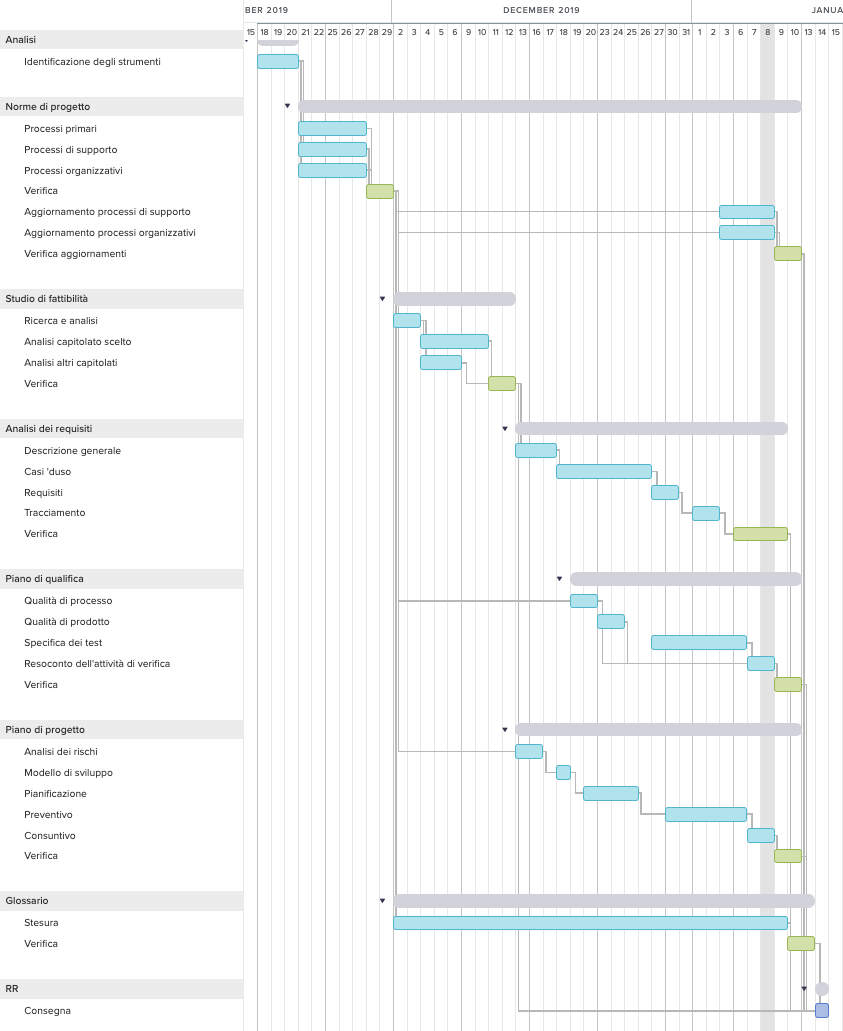
\includegraphics[width=\textwidth]{res/img/g1113}
	\caption{Pianificazione - Analisi dei requisiti}
\end{figure}
Questo periodo è composto dalle seguenti attività:
\begin{itemize}
	\item \textbf{Individuazione degli strumenti:} questa attività consiste nel determinare quali strumenti il gruppo deve utilizzare per la comunicazione, per la stesura dei documenti, per il versionamento, lo sviluppo e la verifica del software;
	\item \textbf{Norme di Progetto:} sono definite tutte le regole utili per lo svolgimento del progetto, relative al prodotto da realizzare e ai processi da adottare. Il documento \textit{Norme di Progetto 1.3.1}\doc viene redatto dall'Amministratore per conto del Responsabile di progetto e viene costantemente aggiornato;
	\item \textbf{Studio di fattibilità:} in questa attività gli analisti effettuano uno studio approfondito dei capitolati in modo da determinare quale di essi verrà scelto. Questa attività è da considerarsi bloccante per l’attività di Analisi dei Requisiti;
	\item \textbf{Analisi dei Requisiti:} durante questa attività vengono identificati ed analizzati i requisiti del capitolato scelto nell'attività di studio di fattibilità e il relativo documento viene composto dagli Analisti;
	\item \textbf{Piano di Qualifica:} in questa attività si individuano le metodologie attraverso le quali si garantisce la qualità del prodotto. A supporto di ciò viene redatto il documento Piano di Qualifica da parte dell'Amministratore e per la parte programmatica dal Progettista;
	\item \textbf{Glossario:} tutti i termini che possono risultare ambigui vengono individuati e definiti nel documento \textit{Glossario 1.0.0}\docs, che viene redatto durante tutta l'analisi dei requisiti.
\end{itemize}

\begin{figure}[h!]
	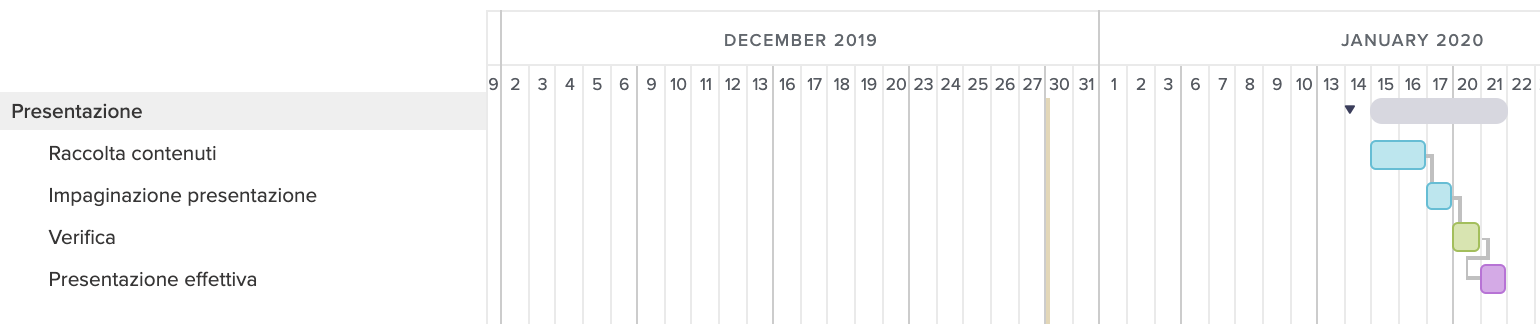
\includegraphics[width=\textwidth]{res/img/g2}
	\caption{Pianificazione presentazione RR}
\end{figure}

\newpage
\subsection{Progettazione architetturale}
Questo periodo ha come obbiettivo l'individualizzazione di una soluzione architetturale che soddisfi i requisiti del prodotto ed è stata suddiviso nelle attività:
\begin{itemize}
	\item \textbf{Technology \textit{Baseline\glos}:} redazione di un documento nel quale vengono individuati e specificati i pattern architetturali utilizzati negli ambiti delle tecnologie coinvolte;
	\item  \textbf{Proof of concept:} codifica di una bozza del prodotto per verificare la correttezza dell'architettura del sistema;
	\item \textbf{Documentazione:} incremento della documentazione in base ai nuovi dati rilevati.
\end{itemize}
\subsubsection{Proof Of Concept}
Sono state identificate tre aree di interesse tecnologico principali:
\begin{itemize}
	\item \textbf{Smart contract}: contratto Ethereum\glo, fulcro del funzionamento di \textit{Etherless};
	\item \textbf{Comunicazione tra client e server}: applicativo client e server devono scambiarsi dati attraverso lo smart contract;
	\item \textbf{Serverless\glo}: ambiente server convertito in ambiente serverless\glos.
\end{itemize}
Questi Proof Of Concept saranno la base della costruzione dei componenti finali di \textit{Etherless}, ovvero \textit{eth-smart, eth-client, eth-server}.
\subsubsection{Incrementi previsti - scadenze}
\begin{itemize}
	\item \textbf{\RomanNumeralCaps{1} Incremento:} entro il 2020-02-19;
	\item \textbf{\RomanNumeralCaps{2} Incremento:} entro il 2020-02-25;
	\item \textbf{\RomanNumeralCaps{3} Incremento:} entro il 2020-02-28;
	\item \textbf{\RomanNumeralCaps{4} Incremento:} entro il 2020-03-05;
	\item \textbf{\RomanNumeralCaps{5} Incremento:} entro il 2020-03-09;
	\item \textbf{\RomanNumeralCaps{6} Incremento:} entro il 2020-03-16.
\end{itemize}
	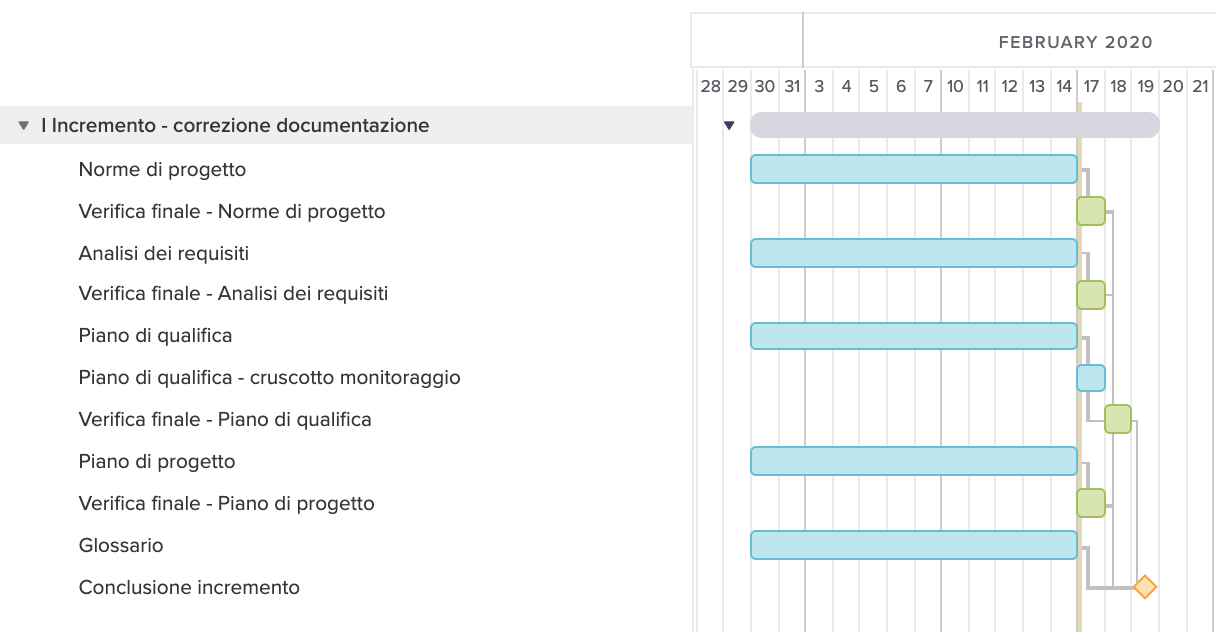
\includegraphics[width=\textwidth]{res/img/gantt/RP/1}
	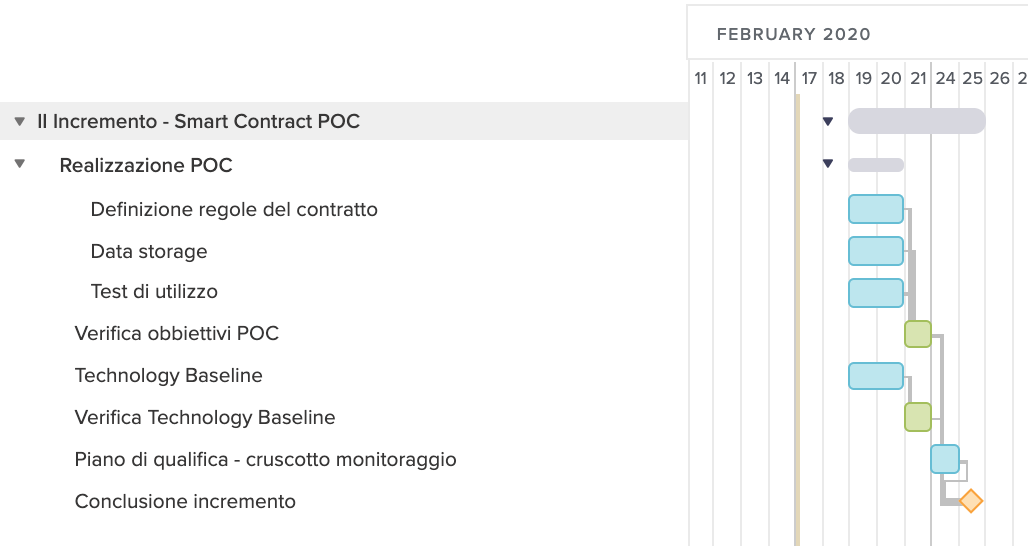
\includegraphics[width=\textwidth]{res/img/gantt/RP/2}
	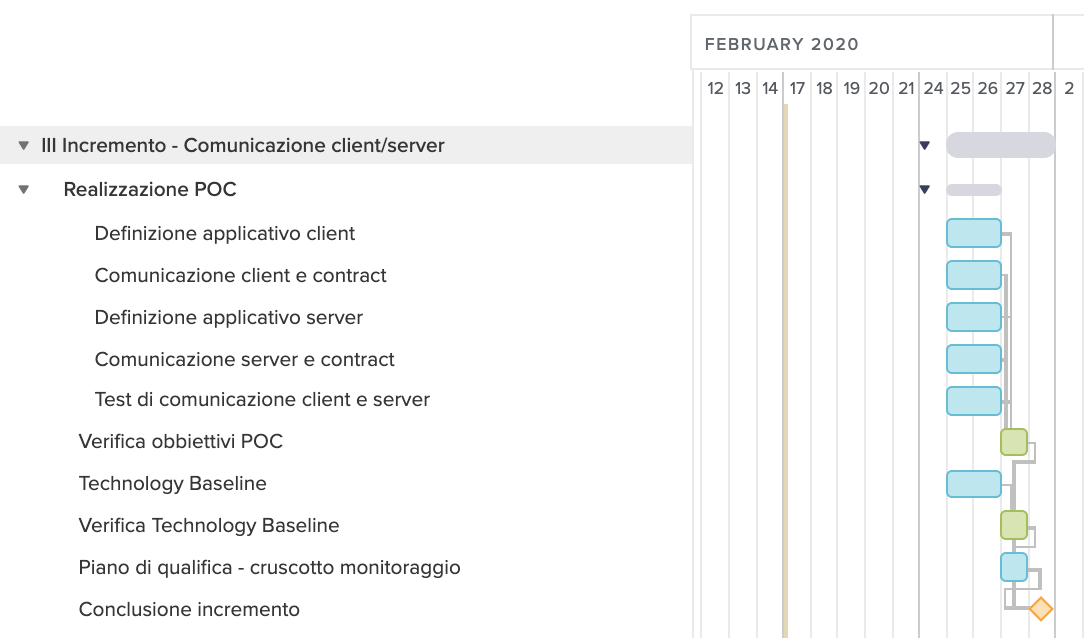
\includegraphics[width=\textwidth]{res/img/gantt/RP/3}
	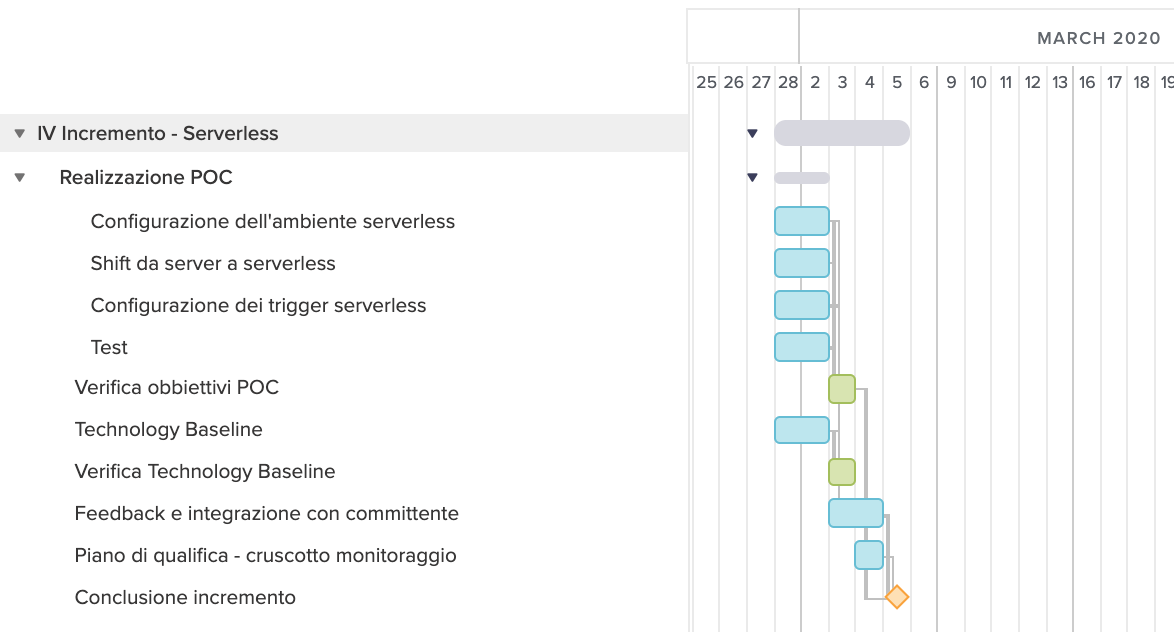
\includegraphics[width=\textwidth]{res/img/gantt/RP/4}
	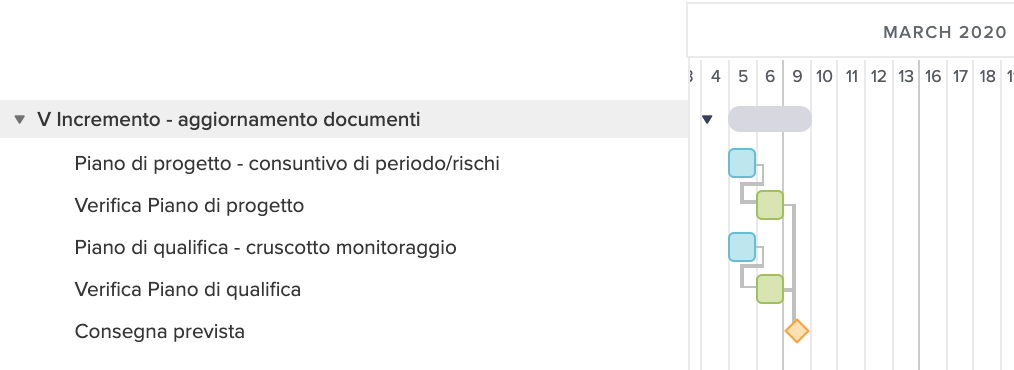
\includegraphics[width=\textwidth]{res/img/gantt/RP/5}
	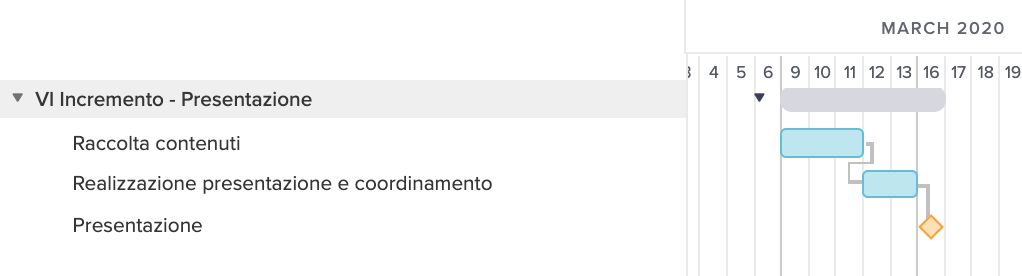
\includegraphics[width=\textwidth]{res/img/gantt/RP/6}
\begin{figure}[h!]
	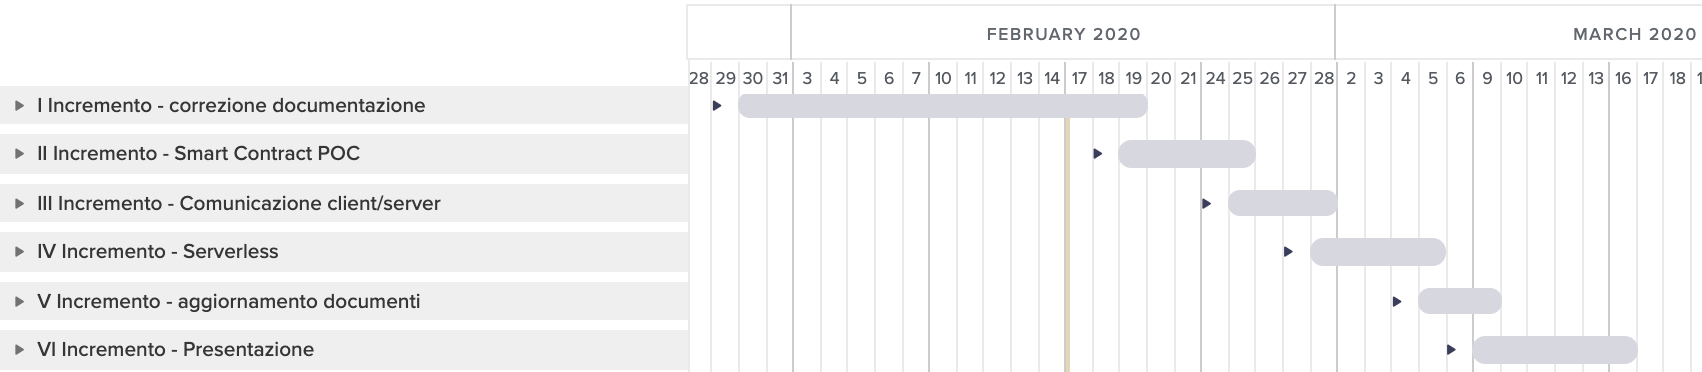
\includegraphics[width=\textwidth]{res/img/gantt/RP/f}
	\caption{Pianificazione Progettazione architetturale}
\end{figure}
\newpage
\subsection{Progettazione di dettaglio e codifica}

\noindent Questo periodo è stata suddiviso nelle attività:
\begin{itemize}
	\item \textbf{Specifiche di prodotto:} documento nel quale vengono individuate le unità che costituiscono il prodotto; viene eseguita una progettazione dettagliata in modo da permettere la successiva codifica delle funzionalità;
	\item  \textbf{Codifica:} implementazione del prodotto;
	\item \textbf{Manuale utente:} realizzazione del \textit{Manuale Utente} per l'utilizzo del prodotto;
	\item \textbf{Documentazione:} incremento della documentazione in base ai nuovi dati rilevati.
\end{itemize}
\subsubsection{Componenti}
Per la realizzazione del prodotto software è necessaria la codifica e la completa conformità di \textit{eth-smart, eth-client, eth-server} ai requisiti del committente e ai casi d'uso.\\
	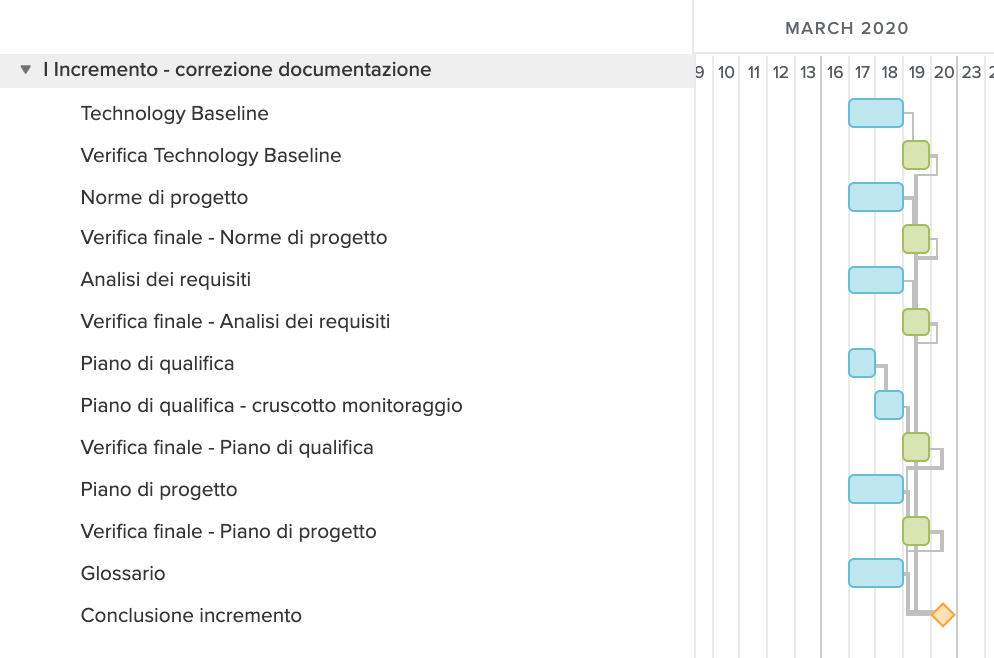
\includegraphics[width=\textwidth]{res/img/gantt/RQ/1}
	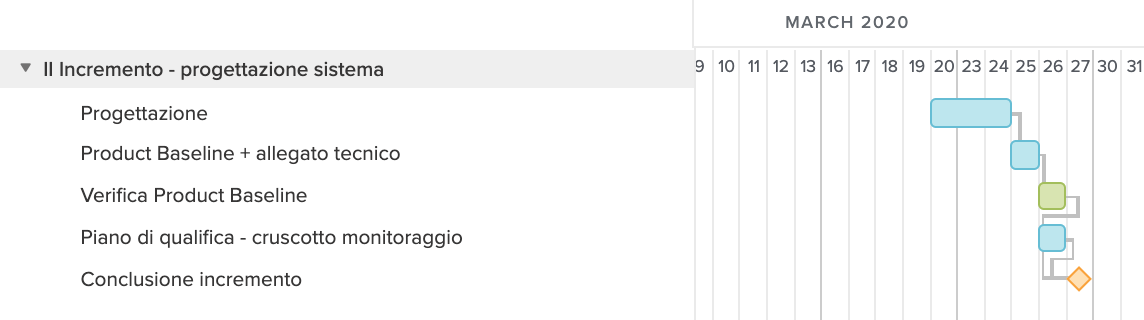
\includegraphics[width=\textwidth]{res/img/gantt/RQ/2}
	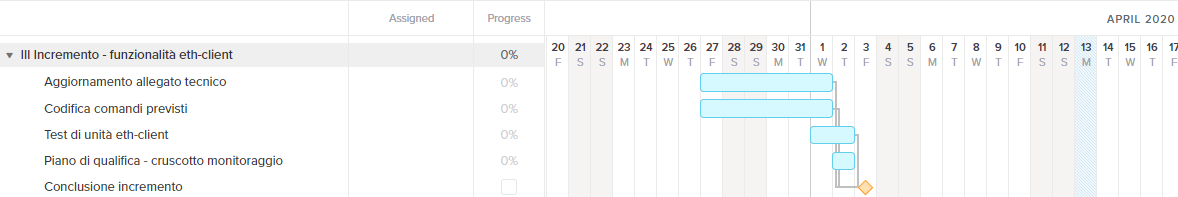
\includegraphics[width=\textwidth]{res/img/gantt/RQ/3}
	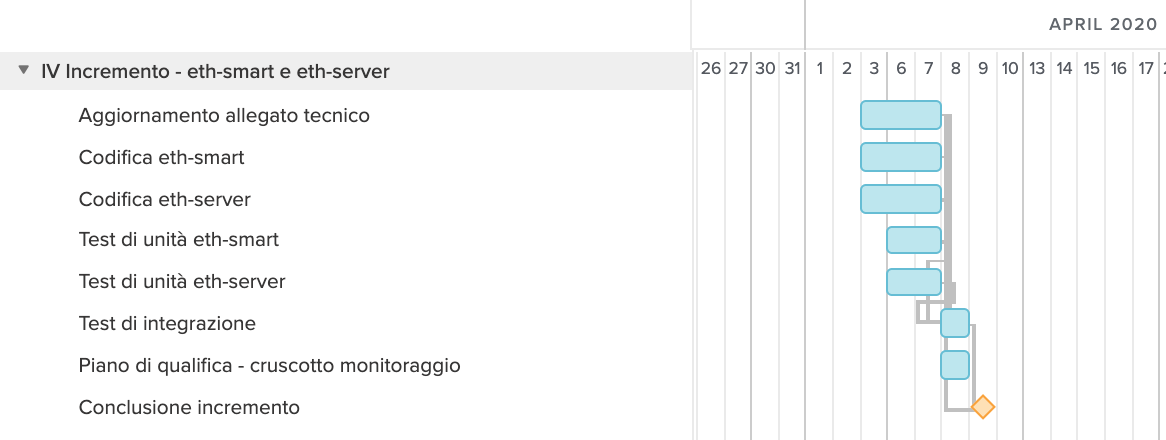
\includegraphics[width=\textwidth]{res/img/gantt/RQ/4}
	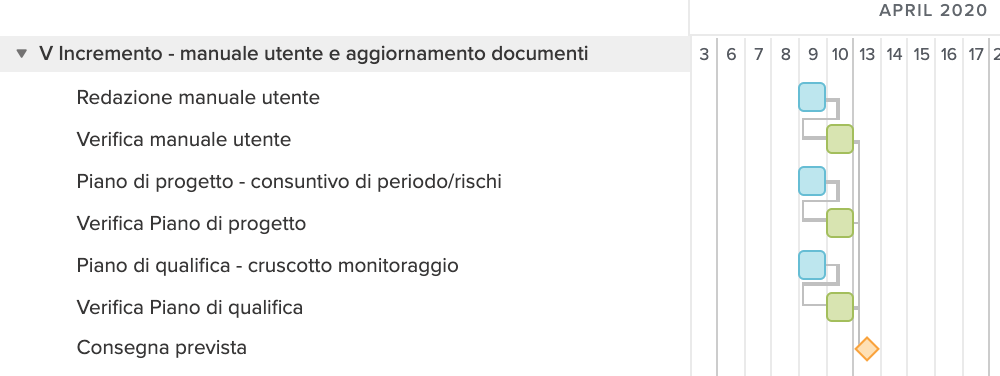
\includegraphics[width=\textwidth]{res/img/gantt/RQ/5}
	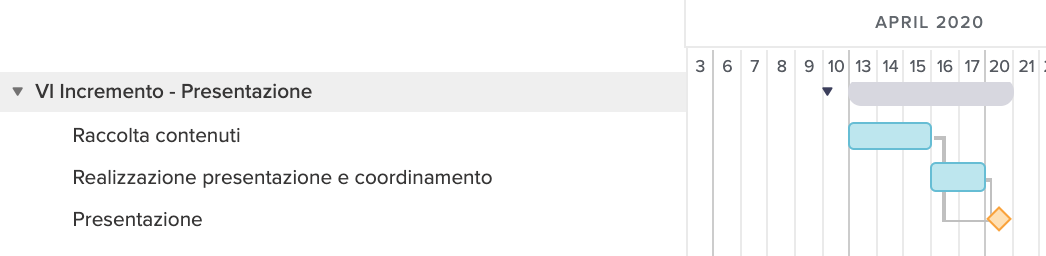
\includegraphics[width=\textwidth]{res/img/gantt/RQ/6}
\begin{figure}[h!]
	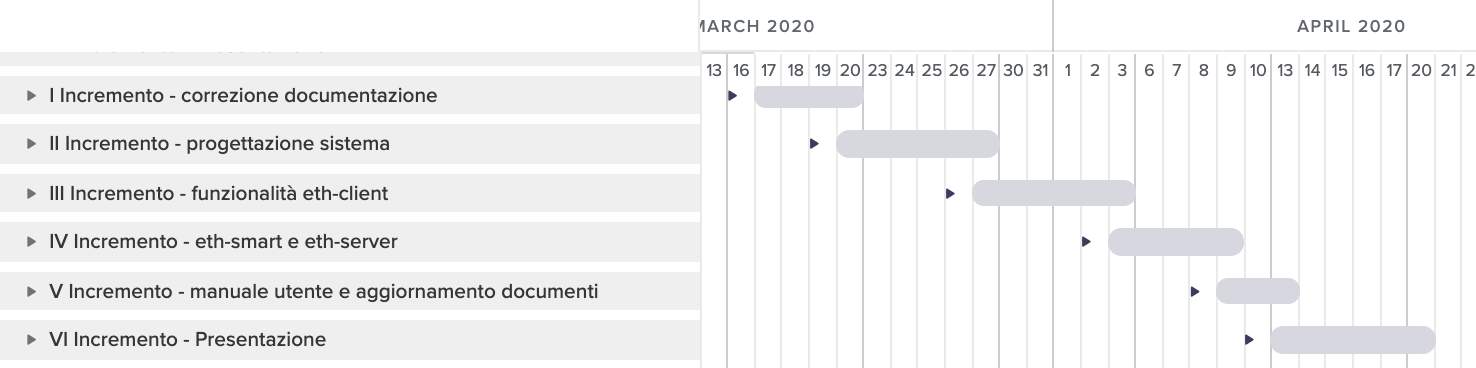
\includegraphics[width=\textwidth]{res/img/gantt/RQ/f}
	\caption{Pianificazione Progettazione di dettaglio}
\end{figure}
\subsubsection{Incrementi previsti - scadenze}
\begin{itemize}
	\item \textbf{\RomanNumeralCaps{1} Incremento:} entro il 2020-03-23;
	\item \textbf{\RomanNumeralCaps{2} Incremento:} entro il 2020-03-27;
	\item \textbf{\RomanNumeralCaps{3} Incremento:} entro il 2020-04-03;
	\item \textbf{\RomanNumeralCaps{4} Incremento:} entro il 2020-04-09;
	\item \textbf{\RomanNumeralCaps{5} Incremento:} entro il 2020-04-13;
	\item \textbf{\RomanNumeralCaps{6} Incremento:} entro il 2020-04-20.
\end{itemize}
\subsection{Validazione e collaudo}
Questo periodo è stati suddiviso nelle attività:
\begin{itemize}
	\item \textbf{Codifica:} modifica del codice se necessario apportare correzioni;
	\item \textbf{Documentazione codice:} realizzazione della documentazione relativa al codice scritto, con lo scopo di fornire informazioni necessarie alla manutenzione del software;
	\item \textbf{Validazione e Collaudo:} controlli per verificare la conformità alle del prodotto ai bisogni del cliente;
	\item \textbf{Documentazione:} incremento della documentazione in base ai nuovi dati rilevati.
\end{itemize}
\subsubsection{Incrementi previsti - scadenze}
\begin{itemize}
	\item \textbf{\RomanNumeralCaps{1} Incremento:} entro il 2020-04-29;
	\item \textbf{\RomanNumeralCaps{2} Incremento:} entro il 2020-05-04;
	\item \textbf{\RomanNumeralCaps{3} Incremento:} entro il 2020-05-07;
	\item \textbf{\RomanNumeralCaps{4} Incremento:} entro il 2020-05-09;
	\item \textbf{\RomanNumeralCaps{5} Incremento:} entro il 2020-05-11;
	\item \textbf{\RomanNumeralCaps{6} Incremento:} entro il 2020-05-28.
\end{itemize}
	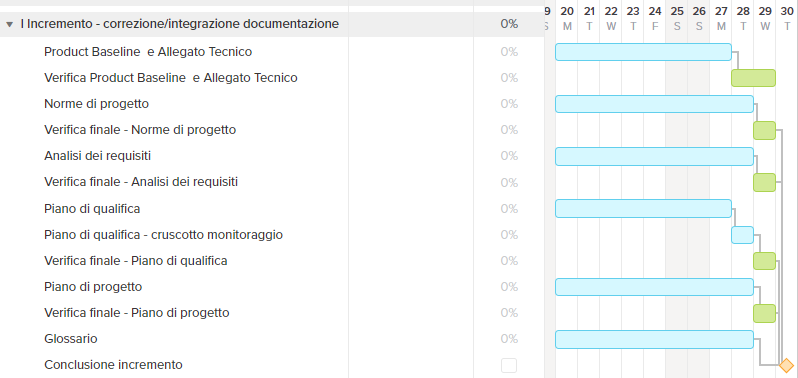
\includegraphics[width=\textwidth]{res/img/gantt/RA/1}
	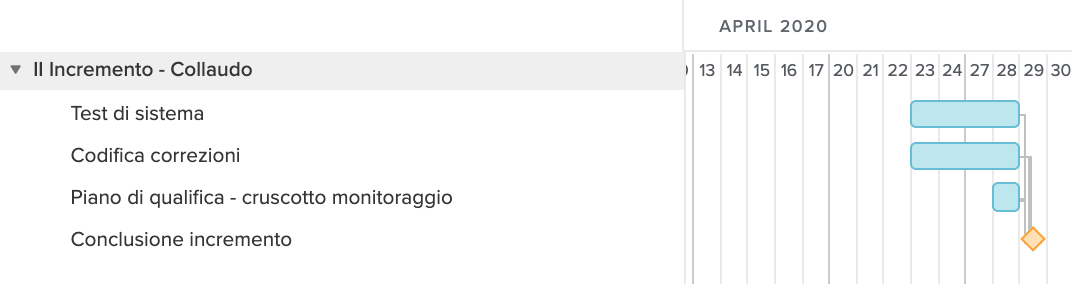
\includegraphics[width=\textwidth]{res/img/gantt/RA/2}
	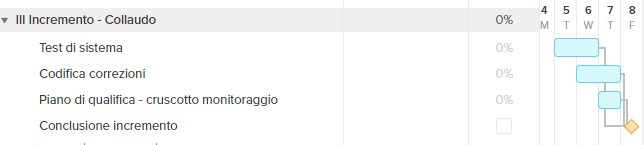
\includegraphics[width=\textwidth]{res/img/gantt/RA/3}
	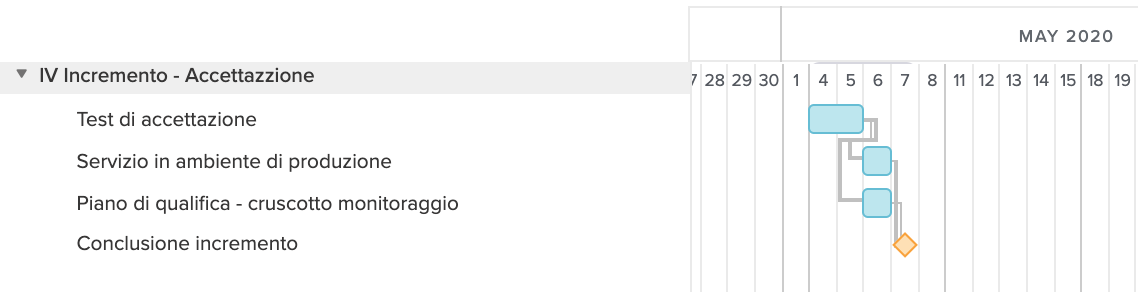
\includegraphics[width=\textwidth]{res/img/gantt/RA/4}
	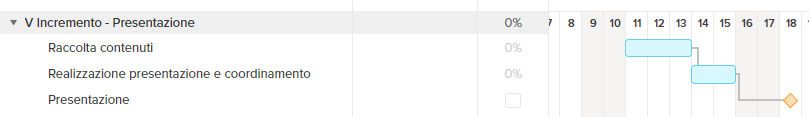
\includegraphics[width=\textwidth]{res/img/gantt/RA/5}
	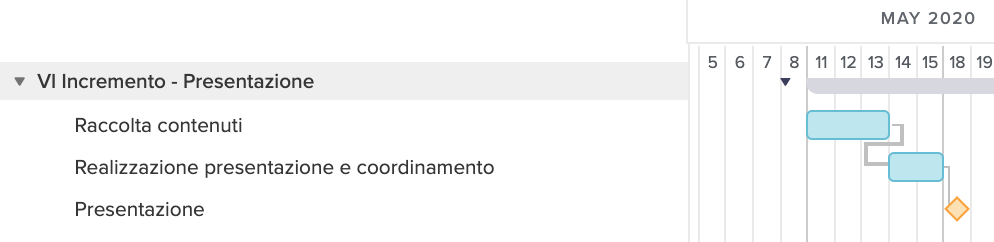
\includegraphics[width=\textwidth]{res/img/gantt/RA/6}
\begin{figure}[h!]
	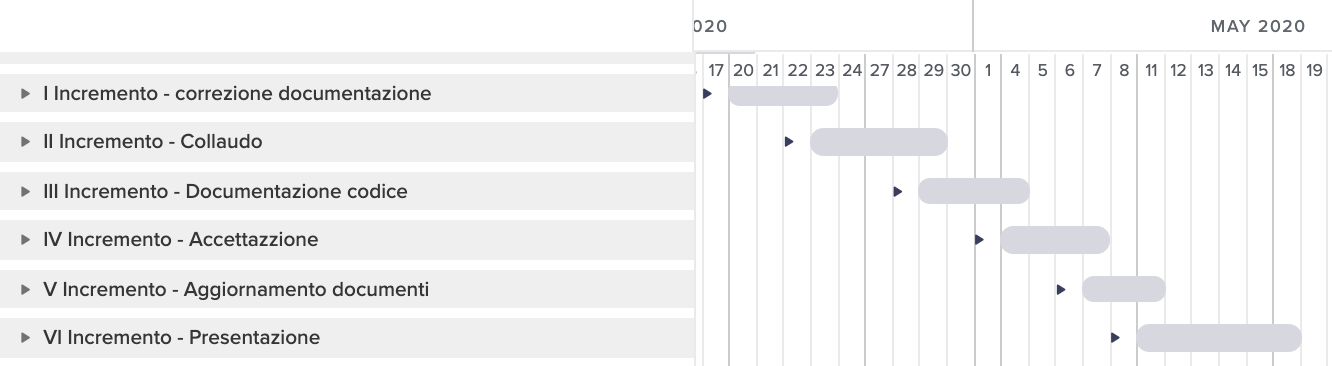
\includegraphics[width=\textwidth]{res/img/gantt/RA/f}
	\caption{Pianificazione Progettazione di dettaglio}
\end{figure}

	\section{Preventivo iniziale}
Verranno utilizzate le seguenti abbreviazioni per indicare i ruoli:
\begin{itemize}
	\item \textbf{RE:} Responsabile;
	\item \textbf{AM:} Amministratore;
	\item \textbf{AN:} Analista;
	\item \textbf{PT:} Progettista;
	\item \textbf{PR:} Programmatore;
	\item \textbf{VE:} Verificatore.
\end{itemize}
Tenners applica le seguenti tariffe per tipo di ruolo coinvolto nell'attività di sviluppo:\\
\begin{table}[h]
\caption{Tabella tariffe per ruolo}            
\begin{center}
\begin{tabular}{ |c|c|  }
 \hline
 Ruolo 		& Tariffa (EUR)\\
 \hline\hline
	Responsabile	& 30\\
	Amministratore	& 20\\
	Analista		& 25\\
	Progettista		& 22\\
	Programmatore	& 15\\
	Verificatore	& 15\\
 \hline
\end{tabular}
\end{center}
\end{table}
\newpage
\subsection{Analisi dei requisiti}
\subsubsection{Prospetto orario}
Il team ha previsto la seguente suddivisione di ruoli durante questo periodo:\\
\begin{table}[h]
\caption{Tabella suddivisione per ruolo, Analisi dei requisiti}  
\begin{center}
\begin{tabular}{ |c|c|c|c|c|c|c|c|  }
 \hline
 Membro 		& RE 	& AM 	& AN 	& PT 	& PR 	& VE 	& Tot.\\
 \hline\hline
 Simone	Franconetti		& 4 		& 4 		& 14 	& 2 		& 0 		& 6 		& 30\\
 Gabriel Ciulei			& 3 		& 2 		& 20 	& 2 		& 0 		& 3 		& 30\\
 Nicola	Salvadore		& 6 		& 4 		& 10 	& 0 		& 0 		& 10 	& 30\\
 Gianmarco	Pettinato	& 0 		& 2 		& 16 	& 2 		& 0 		& 10 	& 30\\
 Gezim	Cikaqi			& 6 		& 10 	 	& 6 		& 2 		& 0 		& 6	 	& 30\\
 Paola	Trevisan		& 6 		& 2 		& 10 	& 2 		& 0 		& 10 	& 30\\
 Giovanni	Incalza		& 6 		& 11 		& 8 		& 0 		& 0 		& 5  	& 30\\
 \hline\hline
 Ore totali		& 31		& 35		& 84 	& 10 	& 0 		& 50 	& 210\\
  \hline
\end{tabular}
\end{center}
\end{table}
\begin{figure}[h!]
	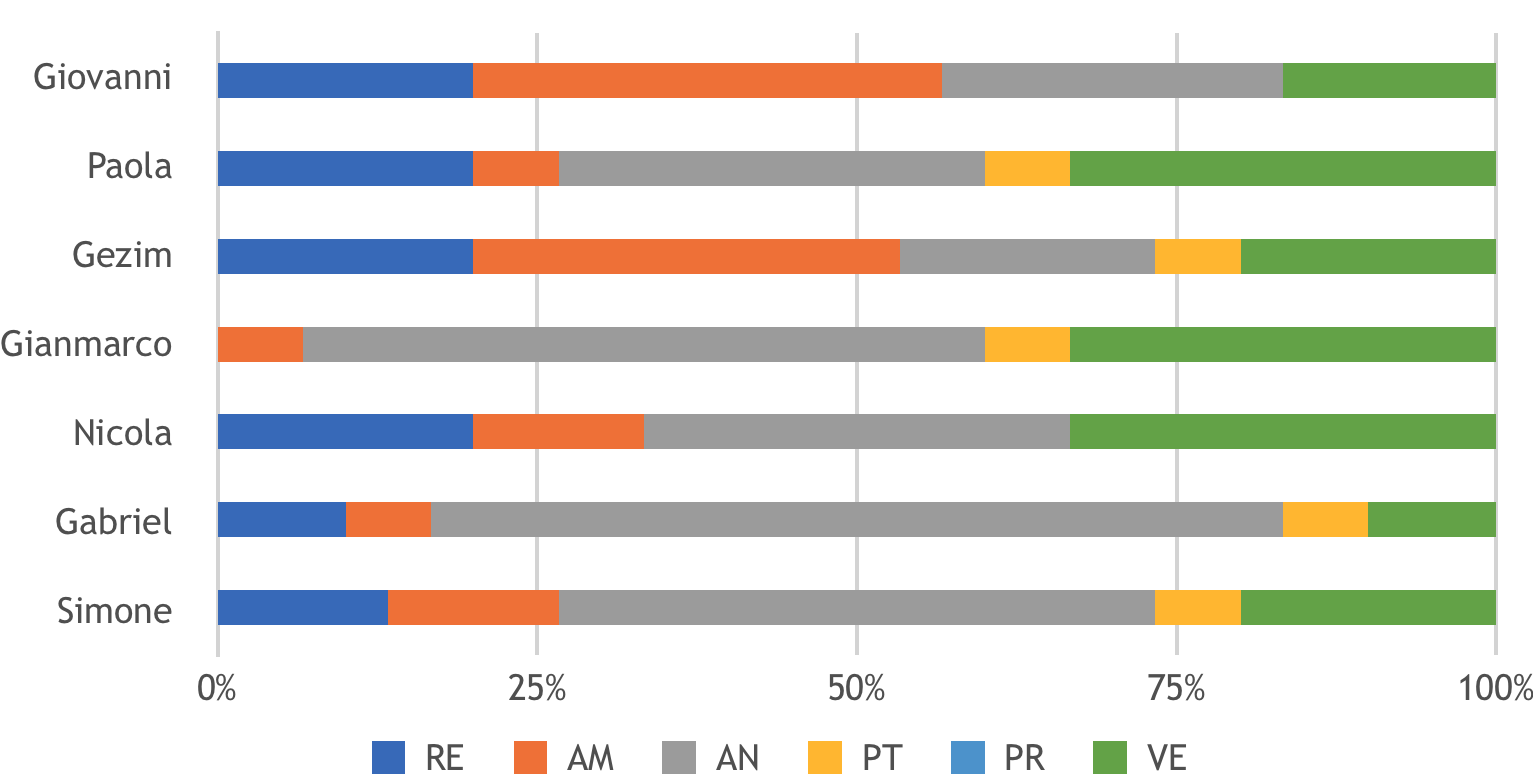
\includegraphics[width=\textwidth]{res/img/hi17}
	\caption{Diagramma della suddivisione dei ruoli, Analisi dei requisiti}
\end{figure}

\noindent Viene riportato in seguito, a solo scopo informativo, il valore economico complessivo che il team Tenners ha deciso di investire in questo periodo.
\noindent \textbf{Si ricorda infatti che il lavoro sostenuto durante questo periodo non viene rendicontato nei confronti del cliente.} \\
Il valore economico totale investito è di 4.700,00 EUR.
\begin{table}[h]
	\caption{Tabella prospetto economico, Analisi dei requisiti}  
\begin{center}
\begin{tabular}{ |c|c|c|  }
 \hline
 Ruolo 		& Ammontare ore 	& Totale (EUR)\\
 	\hline
 \hline
 	Responsabile	& 31 	& 930\\
	Amministratore	& 35		& 700\\
	Analista		& 84 	& 2100\\
	Progettista		& 10		& 220\\
	Programmatore	& 0		& 0\\
	Verificatore	& 50		& 750\\
 \hline\hline
 TOTALE		& 210		& 4700\\
  \hline
\end{tabular}
\end{center}
\end{table}
\newpage
\subsection{Progettazione architetturale}
\subsubsection{Prospetto orario}
Il team ha previsto la seguente suddivisione di ruoli per questa periodo:
\\
\begin{table}[h]
\caption{Tabella suddivisione per ruolo, Progettazione architetturale}  
\begin{center}
\begin{tabular}{ |c|c|c|c|c|c|c|c|  }
 \hline
 Membro 		& RE 	& AM 	& AN 	& PT 	& PR 	& VE 	& Tot.\\
 \hline\hline
 Simone	Franconetti		& 5 		& 0		& 6 	& 13 	& 6 		& 0 		& 30\\
 Gabriel Ciulei		& 0 		& 5 		& 2 	& 15		& 8 		& 0 		& 30\\
 Nicola	Salvadore		& 0 		& 2 		& 4 	& 8		& 8 		& 8 		& 30\\
 Gianmarco	Pettinato	& 5 		& 8 		& 3 	& 10 	& 2 		& 2 		& 30\\
 Gezim	Cikaqi		& 0 		& 0 		& 10 	& 10		& 4 		& 6	 	& 30\\
 Paola	Trevisan		& 0 		& 4 		& 6 	& 8 		& 6 		& 6 		& 30\\
 Giovanni Incalza		& 0 		& 0	 	& 8 	& 10		& 4 		& 8  	& 30\\
 \hline\hline
 Ore totali		& 10		& 19		& 39 	& 74	 	& 38 	& 30 	& 210\\
  \hline
\end{tabular}
\end{center}
\end{table}
\begin{figure}[h!]
	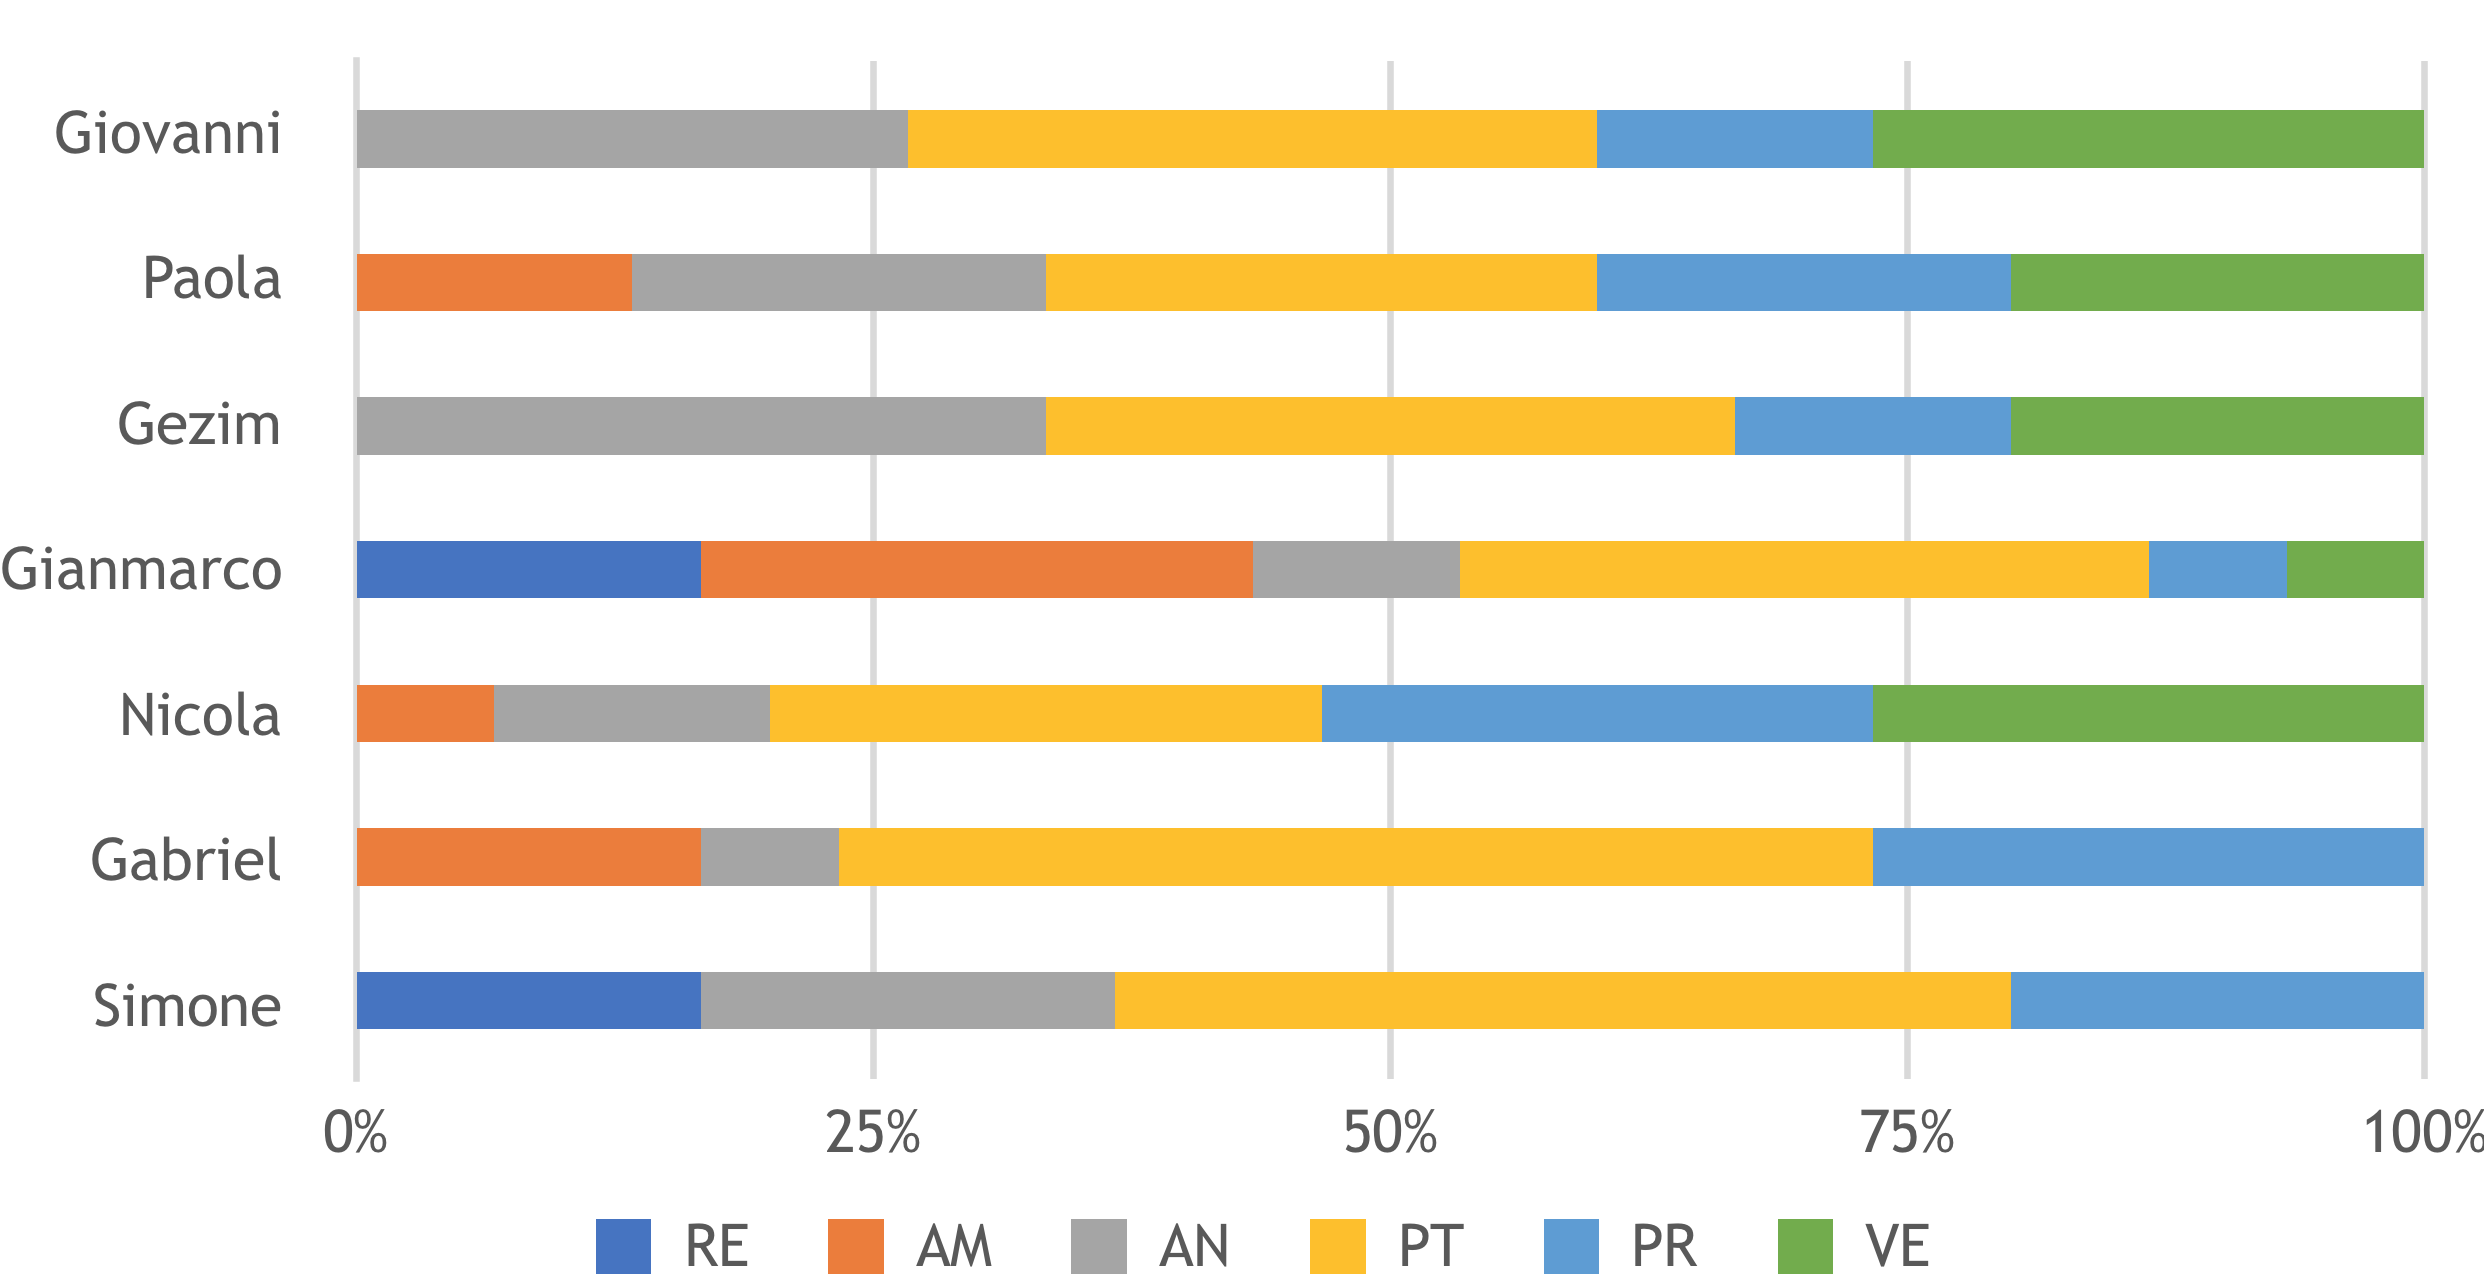
\includegraphics[width=0.9\textwidth]{res/img/hi336}
	\caption{Diagramma della suddivisione dei ruoli, Progettazione architetturale}
\end{figure}

\noindent Vengono inoltre dettagliate in seguito le ore previste per portare a termine ciascun incremento del prodotto durante il periodo di Progettazione architetturale:

\begin{table}[h]
	\caption{Tabella ore previste per incremento, Progettazione architetturale}  
	\begin{center}
		\begin{tabular}{ |c|c|c|c|c|c|c|c|  }
			\hline
			Incremento 		& RE 	& AM 	& AN 	& PT 	& PR 	& VE 	& Tot.\\
			\hline\hline
			I		& 2 		& 9			& 8 	& 40 	& 0 		& 10 		& 69\\
			II		& 1 		& 1 		& 8 	& 10	& 14 		& 3 		& 37\\
			III		& 1 		& 2 		& 8 	& 10	& 14 		& 3 		& 38\\
			IV		& 2 		& 2 		& 8 	& 10 	& 10 		& 3 		& 35\\
			V		& 3 		& 3 		& 5 	& 4		& 0 		& 8	 		& 23\\
			VI		& 1 		& 2 		& 2 	& 0 	& 0 		& 3 		& 8\\
			\hline\hline
			Ore totali		& 10		& 19		& 39 	& 74	 	& 38 	& 30 	& 210\\
			\hline
		\end{tabular}
	\end{center}
\end{table}

\subsubsection{Prospetto economico}
In base alle ore necessarie per il completamento di questo periodo, il valore economico totale è di 4.303,00 EUR.
\begin{table}[h]
	\caption{Tabella prospetto economico, Progettazione architetturale}  
\begin{center}
\begin{tabular}{ |c|c|c|  }
 \hline
 Ruolo 		& Ammontare ore 	& Totale (EUR)\\
 	\hline
 \hline
 	Responsabile	& 10 	& 300\\
	Amministratore	& 19		& 380\\
	Analista		& 39 	& 975\\
	Progettista		& 74		& 1628\\
	Programmatore	& 38		& 570\\
	Verificatore	& 30 	& 450\\
 \hline\hline
 TOTALE		& 210		& 4303\\
  \hline
\end{tabular}
\end{center}
\end{table}
\newpage
\subsection{Progettazione di dettaglio e codifica}
\subsubsection{Prospetto orario}
Il team ha previsto la seguente suddivisione di ruoli per questo periodo:
\begin{table}[h]
\caption{Tabella suddivisione per ruolo, Progettazione di dettaglio e codifica}  
\begin{center}
\begin{tabular}{ |c|c|c|c|c|c|c|c|  }
 \hline
 Membro 		& RE 	& AM 	& AN 	& PT 	& PR 	& VE 	& Tot.\\
 \hline\hline
 Simone	Franconetti		& 0 		& 8		& 2 	& 10 	& 25 		& 10 		& 55\\
 Gabriel Ciulei		& 5 		& 0 		& 0 	& 10		& 30 		& 10 		& 55\\
 Nicola	Salvadore		& 5 		& 8 		& 3 	& 9 		& 20 		& 10 		& 55\\
 Gianmarco	Pettinato	& 0 		& 0 		& 0 	& 15 	& 30 		& 10 		& 55\\
 Gezim	Cikaqi		& 5 		& 6 		& 0 	& 12 	& 24 		& 8	 		& 55\\
 Paola	Trevisan		& 5 		& 2 		& 3 	& 15 	& 20 		& 10 		& 55\\
 Giovanni	Incalza	& 5 		& 6	 	& 0 	& 10 	& 24 		& 10  		& 55\\
 \hline\hline
 Ore totali		& 25		& 30		& 8 	& 81	 	& 173 	& 68 	& 385\\
  \hline
\end{tabular}
\end{center}
\end{table}
\begin{figure}[h!]
	\centering
	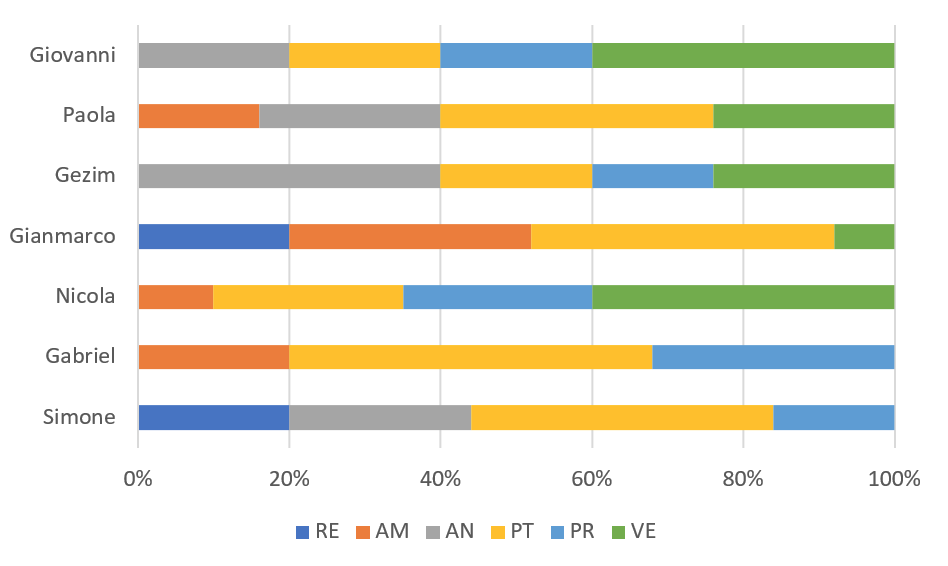
\includegraphics[width=0.9\textwidth]{res/img/hi33}
	\caption{Diagramma della suddivisione dei ruoli, Progettazione di dettaglio e codifica}
\end{figure}

\subsubsection{Prospetto economico}
In base alle ore necessarie per il completamento di questa periodo, il valore economico totale è di 6.947,00 EUR.
\begin{table}[h]
\caption{Tabella prospetto economico, Progettazione di dettaglio e codifica}  
\begin{center}
\begin{tabular}{ |c|c|c|  }
 \hline
 Ruolo 		& Ammontare ore 	& Totale (EUR)\\
 	\hline
 \hline
 	Responsabile	& 25 		& 750\\
	Amministratore	& 30		& 600\\
	Analista		& 8 	& 200\\
	Progettista		& 81		& 1782\\
	Programmatore	& 173		&2595 \\
	Verificatore	& 68 	& 1020\\
 \hline\hline
 TOTALE		& 385		& 6947\\
  \hline
\end{tabular}
\end{center}
\end{table}
\newpage
\subsection{Validazione e Collaudo}
\subsubsection{Prospetto orario}
Il team ha previsto la seguente suddivisione di ruoli per questo periodo:
\begin{table}[h]
\caption{Tabella suddivisione per ruolo, Validazione e Collaudo}  
\begin{center}
\begin{tabular}{ |c|c|c|c|c|c|c|c|  }
 \hline
 Membro 		& RE 	& AM 	& AN 	& PT 	& PR 	& VE 	& Tot.\\
 \hline\hline
 Simone Franconetti			& 4 		& 0		& 0 	& 2 		& 4 		& 10 		& 20\\
 Gabriel Ciulei		& 0 		& 6 		& 0 	& 4		& 2 		& 8 		& 20\\
 Nicola	Salvadore		& 0 		& 0 		& 0 	& 6 		& 4 		& 10 		& 20\\
 Gianmarco Pettinato		& 4 		& 6 		& 0 	& 0	 	& 4 		& 6 		& 20\\
 Gezim Cikaqi			& 0 		& 2 		& 0 	& 0 		& 8 		& 10	 	& 20\\
 Paola Trevisan			& 4 		& 4 		& 0 	& 0 		& 8 		& 4 		& 20\\
 Giovanni Incalza		& 2 		& 0	 	& 0 	& 2 		& 12 	& 4  	& 20\\
 \hline\hline
 Ore totali		& 14		& 18		& 0 	& 14	 	& 42 	& 52 	& 140\\
  \hline
\end{tabular}
\end{center}
\end{table}
\begin{figure}[h!]
	\centering
	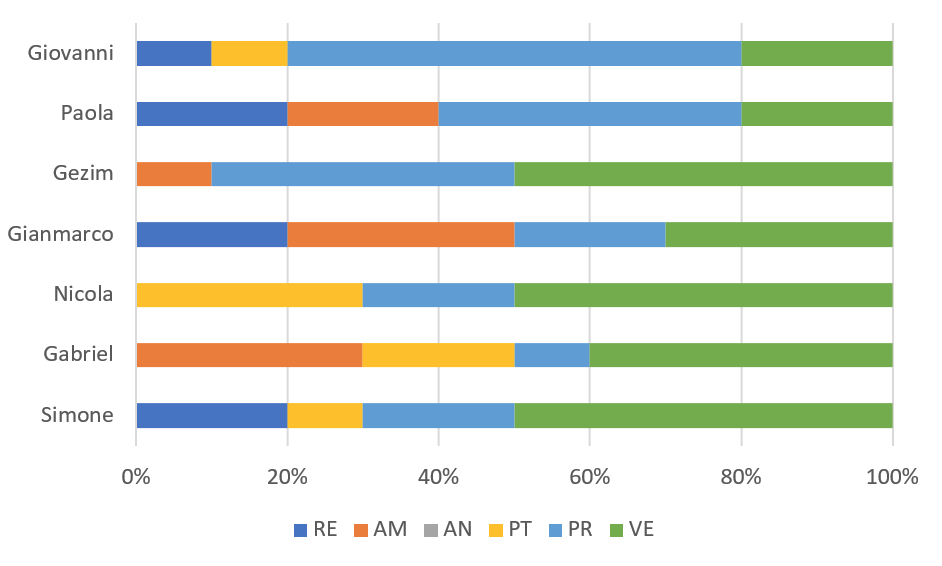
\includegraphics[width=0.9\textwidth]{res/img/hi5}
	\caption{Diagramma della suddivisione dei ruoli, Validazione e Collaudo}
\end{figure}

\subsubsection{Prospetto economico}
In base alle ore necessarie per il completamento di questo periodo, il valore economico totale è di 2.498,00 EUR.
\begin{table}[h]
\caption{Tabella prospetto economico, Verifica e Collaudo}  
\begin{center}
\begin{tabular}{ |c|c|c|  }
 \hline
 Ruolo 		& Ammontare ore 	& Totale (EUR)\\
 \hline
 \hline
 	Responsabile	& 14 	& 420\\
	Amministratore	& 18		& 360\\
	Analista		& 0 		& 0\\
	Progettista		& 14		& 308\\
	Programmatore	& 42		& 630\\
	Verificatore	& 52 	& 780\\
 \hline\hline
 TOTALE		& 140		& 2498\\
  \hline
\end{tabular}
\end{center}
\end{table}
\newpage
\subsection{Totale ore investite}
\subsubsection{Prospetto orario}
Il team ha previsto la seguente suddivisione di ruoli per il completamento del progetto, comprensivo delle ore investite prima dell'ingresso in RR:
\begin{table}[h]
\caption{Tabella di riepilogo del prospetto orario}  
\begin{center}
\begin{tabular}{ |c|c|c|c|c|c|c|c|  }
 \hline
 Membro 		& RE 		& AM 		& AN 	& PT 	& PR 	& VE 	& Tot.\\
 \hline\hline
 Simone	Franconetti		& 13 		& 16			& 23 		& 24 		& 33 		& 26 		& 140\\
 Gabriel Ciulei		& 8 			& 13 		& 22 		& 28		& 40 		& 24 		& 140\\
 Nicola	Salvadore		& 11 		& 14 		& 16 		& 22 		& 32 		& 40 		& 140\\
 Gianmarco Pettinato		& 12 		& 16 		& 18 		& 27	 	& 34 		& 28 		& 140\\
 Gezim Cikaqi		& 11 		& 18 		& 18 		& 19 		& 36 		& 33	 	& 140\\
 Paola Trevisan		& 15 		& 12 		& 24 		& 26 		& 28 		& 30 		& 140\\
 Giovanni	Incalza	& 13 		& 17	 		& 16 		& 17 		& 41	 	& 31  		& 140\\
 \hline\hline
 Ore totali		& 83 	& 106		& 149 	& 179 	& 253 	& 210 	& 980\\
  \hline
\end{tabular}
\end{center}
\end{table}
\begin{figure}[h!]
	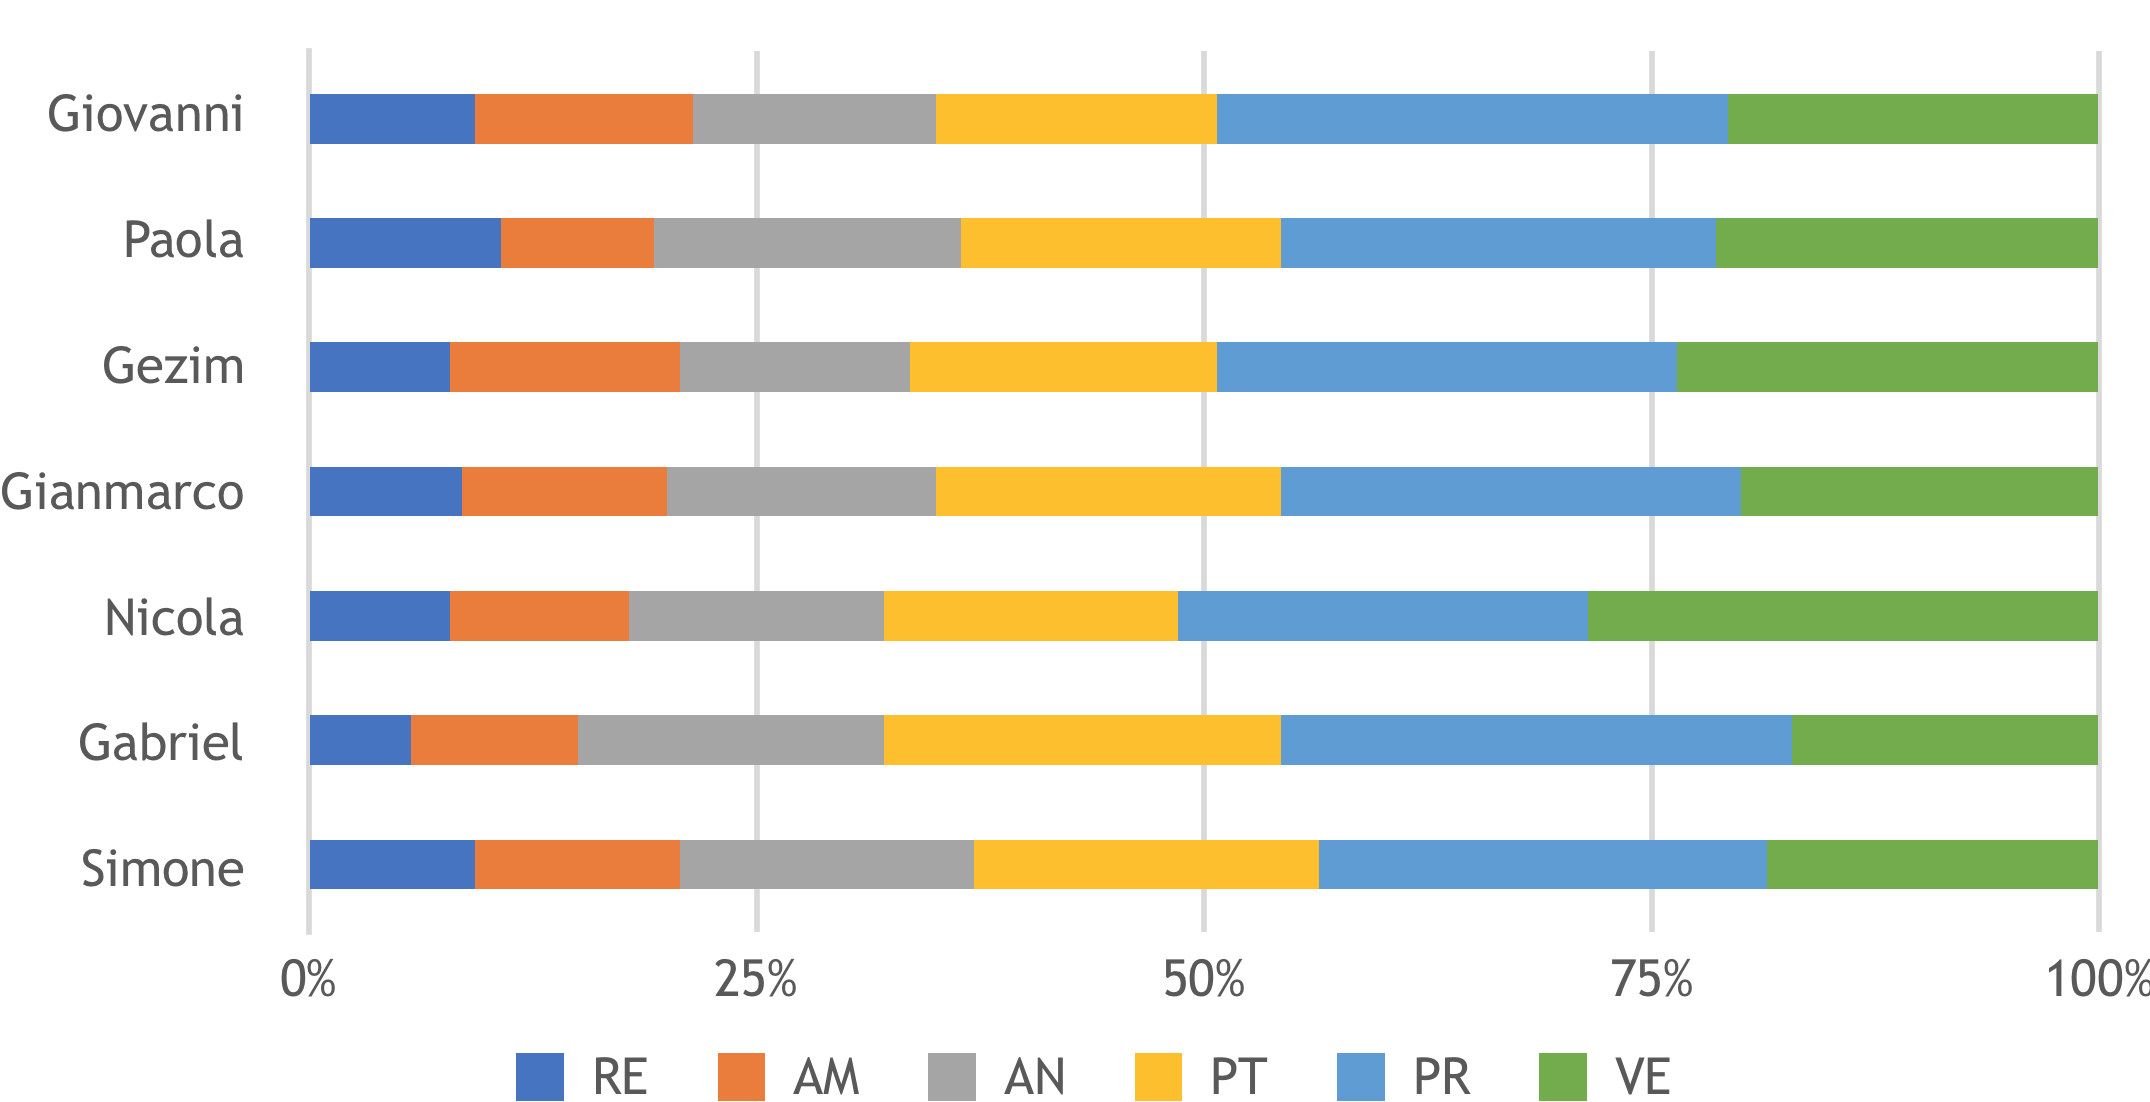
\includegraphics[width=\textwidth]{res/img/hip3}
	\caption{Diagramma della suddivisione dei ruoli durante l'intero il progetto}
\end{figure}

\subsubsection{Prospetto economico}
In base alle ore necessarie per il completamento di questo progetto, il valore economico totale è di 19.218,00 EUR.
\begin{table}[h]
\caption{Tabella di riepilogo del prospetto economico}  
\begin{center}
\begin{tabular}{ |c|c|c|  }
 \hline
 Ruolo 		& Ammontare ore 	& Totale (EUR)\\
 \hline
 \hline
 	Responsabile	& 83 		& 2490\\
	Amministratore	& 106		& 2120\\
	Analista		& 149 		& 3725\\
	Progettista		& 179		& 3938\\
	Programmatore	& 253		& 3795\\
	Verificatore	& 210 		& 3150\\
 \hline\hline
 TOTALE		& 980		& 19218\\
  \hline
\end{tabular}
\end{center}
\end{table}

\newpage
\subsection{Totale ore rendicontate}
\subsubsection{Prospetto orario}
Nello specifico, la programmazione della suddivisione del lavoro prevede la seguente divisione dei ruoli per i singoli membri del team:
\begin{table}[h]
	\caption{Tabella di riepilogo del prospetto orario (escluso il periodo iniziale di \textit{Analisi dei requisiti})} 
\begin{center}
\begin{tabular}{ |c|c|c|c|c|c|c|c|  }
 \hline
 Membro 		& RE 		& AM 		& AN 	& PT 	& PR 	& VE 	& Tot.\\
 \hline\hline
 Simone	Franconetti		& 9  	 	& 8			& 2 		& 25 		& 35 		& 20 		& 105\\
 Gabriel Ciulei		& 5 			& 11 		& 2 		& 29			& 40 		& 18 		& 105\\
 Nicola	Salvadore		& 5  		& 10 		& 7 		& 23 		& 32 		& 28 		& 105\\
 Gianmarco	Pettinato	& 9   		& 14 		& 3 		& 25		 	& 36 		& 18 		& 105\\
 Gezim	Cikaqi		& 5  		& 8  		& 10		& 22 		& 36 		& 24	 	& 105\\
 Paola	Trevisan		& 9  		& 10 		& 9 		& 23 		& 34 		& 20 		& 105\\
 Giovanni	Incalza	& 7  		& 6	 		& 8 		& 22 		& 40		 	& 22  		& 105\\
 \hline\hline
 Ore totali		& 49 	& 67		& 47 	& 169 	& 253 	& 150 	& 735\\
  \hline
\end{tabular}
\end{center}
\end{table}

\newpage
\subsubsection{Prospetto economico}
\begin{table}[h]
	\caption{Tabella di riepilogo del prospetto economico (escluso il periodo iniziale di \textit{Analisi dei requisiti})} 
	\begin{center}
		\begin{tabular}{ |c|c|c|  }
			\hline
			Ruolo 		& Ammontare ore 	& Totale (EUR)\\
			\hline
			\hline
			Responsabile	& 49 	& 1470\\
			Amministratore	& 67		& 1340\\
			Analista		& 47 	& 1175\\
			Progettista		& 169	& 3718\\
			Programmatore	& 253	& 3795\\
			Verificatore	& 150 	& 2250\\
			\hline\hline
			TOTALE		& 735		& 13748\\
			\hline
		\end{tabular}
	\end{center}
\end{table}

\subsubsection{Conclusioni}
In conclusione, il totale preventivato per la realizzazione del progetto \textit{Etherless} è di\\ \textbf{13.748,00 EUR}, valore che rispecchia il numero di ore rendicontabili per ogni figura professionale che verrà coinvolta durante la realizzazione del progetto. 

	\section{Consuntivo di periodo}
A seguito di ogni periodo definito nella sezione precedente viene fatto un confronto tra quanto preventivato e le ore effettivamente impiegate per ricoprire i vari ruoli. In particolare, ci interessa definire una metrica che possa riassumere la differenza di costo preventivata ed effettiva, derivante dal residuo di ore impiegate per ruolo. \\ A tale metrica si possono assegnare tre valori distinti:
\begin{itemize}
	\item \textbf{Positivo:} il quantitativo di tempo impiegato risulta inferiore rispetto a quanto preventivato;
	\item \textbf{Pari:} il quantitativo di tempo impiegato è in linea a quanto preventivato (differenza entro il 2\%);
	\item \textbf{Negativo:} il quantitativo di tempo impiegato risulta superiore rispetto a quanto preventivato.
\end{itemize}
La metrica è anche indice delle capacità del gruppo di prevedere i tempi necessari per le varie attività.
\\Inoltre, per ogni periodo verrà specificato se la data di scadenza per il raggiungimento dell'obbiettivo di tale periodo è stato rispettato.
\newpage
\subsection{Analisi dei requisiti}
\subsubsection{Impiego risorse}
\begin{table}[h]
\caption{Tabella consuntivo di periodo, Analisi dei requisiti}  
\begin{center}
\begin{tabular}{ |c|c|c|  }
 \hline
 Ruolo 		& Ore & Costo (EUR)\\
 \hline\hline
	Responsabile	& 31 (+0) & 930,00 (+0)\\
	Amministratore	& 47 (+12) & 940,00 (+240,00)\\
	Analista		& 99 (+15) & 2.475,00 (+375,00)\\
	Progettista		& 14 (+4) & 308,00 (+88,00)\\
	Programmatore	& 0 (+0) & 0 (+0)\\
	Verificatore	& 46 (-4) & 690,00 (-60,00)\\
	\hline\hline
	Totale prev.	& 210 & 4.700,00 \\
	Totale cons.	& 237 & 5.343,00 \\
	Differenza		& +27 & +643,00 \\
 \hline
\end{tabular}
\end{center}
\end{table}
%\noindent \underline{Si ricorda che il lavoro sostenuto durante questo periodo non viene rendicontato nei confronti} \\
%\underline{del costo per il cliente.}
\subsubsection{Conclusioni}
E' risultato necessario un numero di ore maggiore rispetto a quanto preventivato per raggiungere l'obbiettivo richiesto da questo periodo. La discrepanza oraria maggiore è stata rilevata nei ruoli di Amministratore e Analista. Il team ha riscontrato difficoltà più di quanto previsto nella parte decisionale e di configurazione degli strumenti e procedure da utilizzare durante la realizzazione del progetto.
\\Il bilancio di questo periodo è \textbf{Negativo} rispetto a quanto preventivato, con un surplus di 27 ore e uno scarto economico di +643,00 EUR. Tuttavia, non essendo rendicontato, le ore aggiuntive sono state un investimento che porterà beneficio nel proseguo del progetto. La scadenza temporale prefissata per questo periodo è comunque stata rispettata.

\newpage
\subsection{Progettazione architetturale}
\subsubsection{Impiego risorse}
\begin{table}[h]
\caption{Tabella consuntivo di periodo, Progettazione architetturale}  
\begin{center}
\begin{tabular}{ |c|c|c|  }
 \hline
 Ruolo 		& Ore & Costo (EUR)\\
 \hline\hline
	Responsabile	& 10 (+0) & 300,00 (+0)\\
	Amministratore	& 26 (+0) & 520,00 (+0)\\
	Analista		& 34 (-1) & 850,00 (-25,00)\\
	Progettista		& 71 (-1) & 1.562,00 (-22,00)\\
	Programmatore	& 35 (-2) & 525,00 (-30,00)\\
	Verificatore	& 30 (+0) & 450,00 (+0)\\
	\hline\hline
	Totale prev.	& 210 & 4.284,00 \\
	Totale cons.	& 206 & 4.207,00 \\
	Differenza		& -4 & -77,00 \\
 \hline
\end{tabular}
\end{center}
\end{table}
\newpage
\noindent In particolare, per ciascun incremento previsto, sono state impiegate le seguenti ore con relativi costi:
\begin{table}[h]
	\caption{Tabella ore effettuate per incremento, Progettazione architetturale}  
	\begin{center}
		\begin{tabular}{ |c|c|c|c|c|c|c|c|c|c| }
			\hline
			Incremento 		& RE 	& AM 	& AN 	& PT 	& PR 	& VE 	& Tot. (h)		&Tot.(EUR)\\
			\hline\hline
			I		& 2 		& 3			& 10 	& 2 	& 0 		& 4 		& 21 	&474,00\\
			II		& 2 		& 11 		& 10 	& 26	& 15 		& 9 		& 73 	&1.462,00\\
			III		& 2 		& 5 		& 7 	& 22	& 11 		& 7 		& 54 	&1.089,00\\
			IV		& 2 		& 5 		& 6 	& 20 	& 9 		& 7 		& 49 	&990,00\\
			V		& 1 		& 1 		& 1 	& 1		& 0 		& 2	 		& 6 	&127,00\\
			VI		& 1 		& 1 		& 0 	& 0 	& 0 		& 1 		& 3 	&65,00\\
			\hline\hline
			Totale		& 10		& 26		& 34 	& 71	 	& 35 	& 30 	& 206		&4.207,00\\
			\hline
		\end{tabular}
	\end{center}
\end{table}

\subsubsection{Preventivo a finire}
La seguente tabella ha lo scopo di evidenziare le differenze tra la somma che è stata preventivata e il consuntivo effettivo.
\begin{table}[h]
	\caption{Tabella preventivo a finire}  
	\begin{center}
		\begin{tabular}{ |c|c|c|  }
			\hline
			Periodo 								& Preventivo (EUR) & Consuntivo (EUR)\\
			\hline\hline
			Progettazione architetturale			& 4.284,00 				& 4.207,00\\
			Progettazione di dettaglio e codifica	& 6.966,00 			& -\\
			Validazione e collaudo					& 2.498,00 			& -\\
			\hline\hline
			Totale									& 13.748,00 				& 4.207,00 \\
			\hline
		\end{tabular}
	\end{center}
\end{table}
 

\subsubsection{Conclusioni}
È risultato necessario un numero di ore minore rispetto a quanto preventivato per raggiungere l'obbiettivo richiesto da questo periodo. La discrepanza oraria è risultata simile nei ruoli di Analista, Progettista e Programmatore. Il team ha potuto godere dell'approfondimento risultato nella Analisi, che ha portato ad una migliore ideazione e realizzazione del PoC presentato durante la Technology Baseline.
\\Il bilancio di questa periodo è \textbf{Positivo}, con un guadagno di 4 ore e uno scarto economico di -77 EUR. Anche la scadenza temporale prefissata per questo periodo è stata rispettata.
\subsection{Progettazione di dettaglio e codifica}
\subsubsection{Impiego e risorse}
In seguito è rappresentato il consuntivo del periodo di progettazione di dettaglio e codifica:
\begin{table}[h]
	\caption{Tabella consuntivo di periodo, progettazione di dettaglio e codifica}  
	\begin{center}
		\begin{tabular}{ |c|c|c|  }
			\hline
			Ruolo 		& Ore & Costo (EUR)\\
			\hline\hline
			Responsabile	& 24 (-1) & 720,00 (-30,00)\\
			Amministratore	& 23 & 460,00\\
			Analista		& 12 & 300,00\\
			Progettista		& 76 (-7) & 1.672,00 (-66,00)\\
			Programmatore	& 180 (+6) & 2.700,00 (+60,00)\\
			Verificatore	& 70 (+2) & 1.050,00 (+30)\\
			\hline\hline
			Totale prev.	& 385 & 6.966,00 \\
			Totale cons.	& 385 & 6.902,00 \\
			Differenza		& 0 & -64,00 \\
			\hline
		\end{tabular}
	\end{center}
\end{table}
\noindent In particolare, per ciascun incremento previsto, sono state impiegate le seguenti ore con relativi costi:

\begin{table}[h]
	\caption{Tabella ore e costo totale previsti per incremento, progettazione di dettaglio e codifica}
	\begin{center}
		\begin{tabular}{ |c|c|c|c|c|c|c|c|c|  }
			\hline
			Incremento 		& RE 	& AM 	& AN 	& PT 	& PR 	& VE 	& Tot. (h) & Tot. (EUR) \\
			\hline\hline
			I		& 2 		& 7			& 7 	& 10 	& 22 		& 12 		& 60	 & 1.105,00\\
			II		& 5 		& 4 		& 1 	& 22	& 58 		& 18 		&108	&1.879,00\\
			III		& 5 		& 2 		& 1 	& 11	& 48 		& 12 		& 79	&1.357,00\\
			IV		& 6 		& 4 		& 2 	& 31 	& 51 		& 26 		& 120 	&2.147,00\\
			V		& 5 		& 5 		& 0 	& 0		& 0 		& 1	 		& 11			&265,00\\
			VI		& 1 		& 1 		& 1 	& 2 	& 1 		& 1 		& 7			&149,00\\
			\hline\hline
			Totale		& 24		& 23		& 12 	& 76	 	& 180 	& 70 	& 385 	&6.902,00\\
			\hline
		\end{tabular}
	\end{center}
\end{table}

\subsubsection{Preventivo a finire}
La seguente tabella ha lo scopo di evidenziare le differenze tra la somma che è stata preventivata e il consuntivo effettivo.
\begin{table}[h]
	\caption{Tabella preventivo a finire}  
	\begin{center}
		\begin{tabular}{ |c|c|c|  }
			\hline
			Periodo 								& Preventivo (EUR) & Consuntivo (EUR)\\
			\hline\hline
			Progettazione architetturale			& 4.284,00 				& 4.207,00\\
			Progettazione di dettaglio e codifica	& 6.966,00 			& 6.902,00\\
			Validazione e collaudo					& 2.498,00 			& -\\
			\hline\hline
			Totale									& 13.748,00 				& 11.109,00 \\
			\hline
		\end{tabular}
	\end{center}
\end{table}
\subsubsection{Conclusioni}
Durante il periodo di progettazione di dettaglio e codifica sono state rispettate le ore preventivate però e stato necessario riorganizzare la suddivisione dei ruoli e ore. Sono state risparmiate 7 ore dal ruolo di \textit Progettista, questo principalmente dovuto al ruolo di \textit Programmatore il quale ha impiegato più ore rispetto a quelle preventivate, ci sono state 6 ore di lavoro in più necessarie ad ultimare gli ultimi dettagli dell’applicativo. Sono state necessarie 2 in più per il ruolo di \textit Verificatore per ultimare la verifica dei documenti. Il risultato totale del periodo è stato di 6.902,00 EUR.
\\Il bilancio di questa periodo è \textbf{Pari}, con con un risparmio economico di -64 EUR. Anche la scadenza temporale prefissata per questo periodo è stata rispettata.

\subsubsection{Pianificazione futura}
L'impiego di ore sino ad ora rispettato, consente di non effettuare in maniera preventiva delle correzioni sulla pianificazione precedente. 
	\section{Attualizzazione dei rischi}
\subsection{Analisi dei requisiti}
\subsubsection{Elenco rischi}
\rowcolors{2}{pari}{dispari}
\begin{longtable}{|p{2cm}|p{6cm}|p{6cm}|}
	\arrayrulecolor{white}
	\caption{Tabella attuazione dei rischi, analisi dei requisiti}\\ 
	\hline
	\rowcolor{header}
	\textbf{Rischio} & \textbf{Descrizione} & \textbf{Contromisura adottata} \\
	\hline
	RO1              & Alcune scelte decisionali e la configurazione di strumenti e procedure hanno richiesto più tempo rispetto a quanto previsto & Le tempistiche e le risorse delle attività in questione sono state rivalutate.                                                                                                   \\
	RO3              & Tutti i membri del gruppo hanno dovuto sostenere esami e questo ha portato tempi morti per il progetto                      & Riassegnazione delle attività prioritarie ad altri membri.                                                                                                                        \\
	RI1              & Difficoltà nel trovare un ambiente adeguato per le riunioni                                                                 & Ricerca in anticipo di locali adeguati.                                                                                                                                          \\
	RO4              & Alcuni membri lavorano e hanno un disponibilità limitata rispetto agli altri                                                & Comunicazione degli interessati delle proprie indisponibilità periodiche; le impegni in cui è richiesta la presenza del gruppo al completo vengono comunicate con largo anticipo. \\
	RO2              & Il consuntivo del primo periodo di lavoro è più dispendioso rispetto al preventivo                                          & Analisi delle problematiche che hanno portato a questa discrepanza; nessuna comunicazione al committente perché questo primo periodo è un investimento della nostra azienda.     
\end{longtable}


\newpage
\subsection{Progettazione architetturale}
\subsubsection{Elenco rischi}
\begin{longtable}{|p{2cm}|p{6cm}|p{6cm}|}
	\arrayrulecolor{white}
	\caption{Tabella attuazione dei rischi, progettazione architetturale} \\
	\hline
	\rowcolor{header}
	\textbf{Rischio} & \textbf{Descrizione} & \textbf{Contromisura adottata} \\
	\hline
	RA2              & L'inesperienza del team ha portato alla errata stesura di alcune parti dei documenti & Il team ha rivisto gli errori commessi; questi sono statti corretti da subito in modo da limitare i danni.
	\\
	RO4 & Periodo di non disponibilità di un membro a causa di impegni personali & Riassegnazione di attività e scadenze in base agli impegni personali.
	\\
	RI3 & Possono insorgere contrasti e tensioni tra i membri & Il gruppo al completo ha discusso e democraticamente è stata presa una decisione.
\end{longtable}



\newpage
\subsection{Progettazione in dettaglio e codifica}
\subsubsection{Elenco rischi}
\rowcolors{2}{pari}{dispari}
\begin{longtable}{|p{2cm}|p{6cm}|p{6cm}|}
	\arrayrulecolor{white}
	\caption{Tabella attuazione dei rischi, progettazione in dettaglio e codifica} \\
	\hline
	\rowcolor{header}
	\textbf{Rischio} & \textbf{Descrizione} & \textbf{Contromisura adottata} \\
	\hline
	RT1 & La maggior parte delle tecnologie necessarie per la realizzazione del prodotto sono sconosciute ai membri del team & Il team ha risolto questa situazione dividendosi in 3 gruppi e i membri inesperti con le tecnologie sono stati aiutati da quelli che ne erano già a conoscenza\\
	RT2 & Problemi legati alla connessione Internet, che durante gli incontri possono impedire le comunicazioni & Le riunioni più rilevanti vengono registrate e caricate privatamente sul canale YouTube di Tenners, in modo da essere a completa disposizione di qualunque membro che ne avesse bisogno
	\\
	RO4 & Periodo di non disponibilità di un membro a causa di impegni personali & Riassegnazione di attività e scadenze in base agli impegni personali
	\\
	RI3 & Possono insorgere contrasti e tensioni tra i membri & Il gruppo al completo ha discusso e democraticamente è stata presa una decisione\\
	\hline
\end{longtable}


\newpage
\subsection{Validazione e collaudo}
\subsubsection{Elenco rischi}
\rowcolors{2}{pari}{dispari}
\begin{longtable}{|p{2cm}|p{6cm}|p{6cm}|}
	\arrayrulecolor{white}
	\caption{Tabella attuazione dei rischi, validazione e codifica} \\
	\hline
	\rowcolor{header}
	\textbf{Rischio} & \textbf{Descrizione} & \textbf{Contromisura adottata} \\
	\hline
	RT2 & Problemi legati alla connessione Internet, che durante gli incontri possono impedire le comunicazioni & Le riunioni più rilevanti vengono registrate e caricate privatamente sul canale YouTube di Tenners, in modo da essere a completa disposizione di qualunque membro che ne avesse bisogno
	\\
	RO4 & Periodo di non disponibilità di un membro a causa di impegni personali & Riassegnazione di attività e scadenze in base agli impegni personali\\
	\hline
\end{longtable}
	\appendix
	\section{Organigramma}
\subsection{Redazione}
\renewcommand{\arraystretch}{2.2}
\rowcolors{2}{pari}{dispari}
\begin{longtable}{|p{5cm}|c|c|}
	\arrayrulecolor{white}
	\caption{Redazione} \\
	\hline
	\rowcolor{header}
	\textbf{Nominativo} & \centering{\textbf{Data di redazione}} & \textbf{Firma} \\
	\hline
	Gabriel Ciulei & 2020-01-08 & 
\includegraphics[width=0.1\textwidth]{res/img/firme/Gabriel.png} \\
	Simone Franconetti & 2020-01-08 & 
\includegraphics[width=0.2\textwidth]{res/img/firme/Simone.png} \\
	Paola Trevisan & 2020-01-08 & 
\includegraphics[width=0.2\textwidth]{res/img/firme/Paola.png}\\
	\hline
\end{longtable}

\subsection{Approvazione}
\rowcolors{2}{pari}{dispari}
\begin{longtable}{|p{5cm}|c|c|}
	\arrayrulecolor{white}
	\caption{Approvazione} \\
	\hline
	\rowcolor{header}
	\textbf{Nominativo} & \centering{\textbf{Data di approvazione}} & \textbf{Firma} \\
	\hline
	Giovanni Incalza & 2020-01-10 & 
\includegraphics[width=0.2\textwidth]{res/img/firme/Giovanni.png} \\
	Riccardo Cardin & & \\
	Tulio Vardanega  & & \\
	\hline
\end{longtable}
\newpage
\subsection{Accettazione dei componenti}
\rowcolors{2}{pari}{dispari}
\begin{longtable}{|p{5cm}|c|c|}
	\arrayrulecolor{white}
	\caption{Accettazione dei componenti} \\
	\hline
	\rowcolor{header}
	\textbf{Nominativo} & \centering{\textbf{Data di accettazione}} & \textbf{Firma}
	\tabularnewline
	\endfirsthead
	\hline
	Gezim Cikaqi & 2020-01-10 & 
\includegraphics[width=0.2\textwidth]{res/img/firme/Gezim.png} \\
	Gabriel Ciulei & 2020-01-10 & 
\includegraphics[width=0.2\textwidth]{res/img/firme/Gabriel.png} \\
	Simone Franconetti & 2020-01-10 & 
\includegraphics[width=0.2\textwidth]{res/img/firme/Simone.png} \\
	Giovanni Incalza & 2020-01-10 & 
\includegraphics[width=0.2\textwidth]{res/img/firme/Giovanni.png} \\
	Gianmarco Pettinato & 2020-01-10 &  
\includegraphics[width=0.2\textwidth]{res/img/firme/Gianmarco.png} \\
	Nicola Salvadore & 2020-01-10 & 
\includegraphics[width=0.2\textwidth]{res/img/firme/Nicola.png} \\
	Paola Trevisan & 2020-01-10 & 
\includegraphics[width=0.2\textwidth]{res/img/firme/Paola.png}\\
	\hline
\end{longtable}

\subsection{Componenti}
\rowcolors{2}{pari}{dispari}
\begin{longtable}{|p{5cm}|c|c|}
	\arrayrulecolor{white}
	\caption{Componenti} \\
	\hline
	\rowcolor{header}
	\textbf{Nominativo} & \textbf{Matricola} & \textbf{Email}
	\tabularnewline
	\endfirsthead
	\hline
	Gezim Cikaqi & 1069255 & gezim.cikaqi@studenti.unipd.it \\
	Gabriel Ciulei & 1169766 & gabriel.ciulei@studenti.unipd.it\\
	Simone Franconetti & 1143567 & simone.franconetti@studenti.unipd.it\\
	Giovanni Incalza & 1143147 & giovanni.incalza@studenti.unipd.it\\
	Gianmarco Pettinato & 1068299 & gianmarco.pettinato@studenti.unipd.it\\
	Nicola Salvadore & 1143452 & nicola.salvadore@studenti.unipd.it\\
	Paola Trevisan & 1143253 & paola.trevisan.5@studenti.unipd.it\\
	\hline
\end{longtable}
\end{document}
